% !TeX program = lualatex
% Presentación del plan de tesis. Compilar con latexmk -lualatex.
\documentclass[aspectratio=169,12pt]{beamer}

\usepackage[spanish,es-nodecimaldot,es-noshorthands]{babel}
\usepackage{fontspec}
\setmainfont{Arial}
\setsansfont{Arial}
\usefonttheme{professionalfonts}
\usepackage{csquotes}
\usepackage{graphicx}
\usepackage{booktabs}
\usepackage{tabularx}
\usepackage{array}
\usepackage{multicol}
\usepackage{tikz}
\usetikzlibrary{arrows.meta,positioning,calc,fit,backgrounds,shapes.geometric}
\usepackage{pgfplots}
\pgfplotsset{compat=1.18}
\usepgfplotslibrary{groupplots}
\usepackage{siunitx}
\sisetup{locale=DE,per-mode=symbol,group-separator={\,},group-minimum-digits=4}
\usepackage[backend=biber,style=apa,sorting=nyt,maxcitenames=2]{biblatex}
\addbibresource{../referencias_plan_tesis.bib}
% En las láminas se muestra una referencia abreviada; DOI y URL completos
% permanecen en el plan y en el repositorio documental.
\AtEveryBibitem{%
  \clearfield{url}%
  \clearfield{urldate}%
  \clearfield{doi}%
  \clearfield{isbn}%
}

\graphicspath{{../imagenes/}{../../examples/kim_2024_154kv_bedding/results_multilayer_research/}}

% ---------------------------------------------------------------------------
% Identidad visual: una sola familia tipográfica y alto contraste.
% ---------------------------------------------------------------------------
\definecolor{unired}{HTML}{9E1B32}
\definecolor{darkblue}{HTML}{123B5D}
\definecolor{midblue}{HTML}{2B6F9F}
\definecolor{lightblue}{HTML}{DCEAF4}
\definecolor{teal}{HTML}{188977}
\definecolor{orange}{HTML}{D97706}
\definecolor{warmgray}{HTML}{F2F1EE}
\definecolor{textgray}{HTML}{30343B}
\definecolor{softred}{HTML}{F4E4E7}
\definecolor{softgreen}{HTML}{E2F1EC}
\definecolor{softorange}{HTML}{F8EBD7}

\setbeamercolor{normal text}{fg=textgray,bg=white}
\setbeamercolor{frametitle}{fg=white,bg=darkblue}
\setbeamercolor{structure}{fg=unired}
\setbeamercolor{alerted text}{fg=unired}
\setbeamercolor{block title}{fg=white,bg=darkblue}
\setbeamercolor{block body}{fg=textgray,bg=lightblue!45}
\setbeamercolor{exampleblock title}{fg=white,bg=teal}
\setbeamercolor{exampleblock body}{fg=textgray,bg=softgreen}
\setbeamercolor{footline}{fg=white,bg=darkblue}

\setbeamerfont{normal text}{size=\fontsize{20.5}{24}\selectfont}
\setbeamerfont{frametitle}{size=\fontsize{20}{22.5}\selectfont,series=\bfseries}
\setbeamerfont{title}{size=\fontsize{25}{29}\selectfont,series=\bfseries}
\setbeamerfont{subtitle}{size=\fontsize{15}{18}\selectfont}
\setbeamerfont{author}{size=\fontsize{17}{20}\selectfont}
\setbeamerfont{institute}{size=\fontsize{13}{16}\selectfont}
\setbeamerfont{block title}{size=\fontsize{18}{21}\selectfont,series=\bfseries}
\setbeamerfont{block body}{size=\fontsize{17}{20}\selectfont}
\setbeamerfont{itemize/enumerate body}{size=\fontsize{19}{22}\selectfont}
\setbeamerfont{itemize/enumerate subbody}{size=\fontsize{16}{19}\selectfont}
\setbeamertemplate{navigation symbols}{}
\setbeamertemplate{items}[circle]
\setbeamertemplate{caption}{\raggedright\insertcaption\par}
\setbeamerfont{caption}{size=\fontsize{8.5}{10}\selectfont}

\setbeamertemplate{frametitle}{%
  \nointerlineskip
  \begin{beamercolorbox}[wd=\paperwidth,ht=0.064\paperheight,dp=0.017\paperheight,leftskip=0.045\paperwidth,rightskip=0.03\paperwidth]{frametitle}
    \usebeamerfont{frametitle}\insertframetitle
  \end{beamercolorbox}
}

\setbeamertemplate{footline}{%
  \leavevmode
  \begin{beamercolorbox}[wd=\paperwidth,ht=0.038\paperheight,dp=0.011\paperheight,leftskip=0.035\paperwidth,rightskip=0.035\paperwidth]{footline}
    \fontsize{8.5}{10}\selectfont
    \insertshorttitle\hfill\insertsectionhead\hfill\insertframenumber/\inserttotalframenumber
  \end{beamercolorbox}
}

\setbeamertemplate{background canvas}{%
  \begin{tikzpicture}[remember picture,overlay]
    \fill[white] (current page.south west) rectangle (current page.north east);
    \fill[unired] (current page.north west) rectangle ([xshift=0.014\paperwidth]current page.south west);
  \end{tikzpicture}%
}

\newcommand{\Imax}{I_{\max}}
\newcommand{\Tmax}{T_{\max}}
\newcommand{\kx}{k(x,y)}
\newcommand{\rhoth}{\rho_{\mathrm{th}}}
\newcommand{\pct}{\%}
\newcommand{\source}[2][\fontsize{7.4}{8.5}\selectfont]{%
  \begin{tikzpicture}[remember picture,overlay]
    \node[anchor=south west,fill=white,fill opacity=0.96,text opacity=1,
      inner xsep=0pt,inner ysep=1.5pt,text width=0.91\paperwidth,align=left,
      font=#1,text=textgray!88]
      at ([xshift=0.045\paperwidth,yshift=0.054\paperheight]current page.south west)
      {\textbf{Fuente:} #2};
  \end{tikzpicture}%
}
\newcommand{\situacionsubyacente}{%
  \begin{tikzpicture}[remember picture,overlay]
    \node[anchor=north west,inner sep=0pt,
      font=\fontsize{9.6}{10.8}\selectfont\bfseries,text=midblue]
      at ([xshift=0.045\paperwidth,yshift=-0.091\paperheight]current page.north west)
      {Situación subyacente.};
  \end{tikzpicture}%
}
\newcommand{\situaciontecnologica}{%
  \begin{tikzpicture}[remember picture,overlay]
    \node[anchor=north west,inner sep=0pt,
      font=\fontsize{9.6}{10.8}\selectfont\bfseries,text=midblue]
      at ([xshift=0.045\paperwidth,yshift=-0.091\paperheight]current page.north west)
      {La situación tecnológica.};
  \end{tikzpicture}%
}
\newcommand{\noexpone}{%
  \begin{tikzpicture}[baseline=(n.base)]
    \node[rounded corners=2pt,fill=warmgray,draw=textgray!35,inner xsep=5pt,inner ysep=2pt,font=\fontsize{9}{10}\selectfont\bfseries,text=textgray] (n) {MATERIAL DE RESPALDO · NO SE EXPONE};
  \end{tikzpicture}%
}
\newcommand{\statcard}[3]{%
  \begin{tikzpicture}
    \node[rounded corners=4pt,draw=#1!65,fill=#1!9,minimum width=0.195\paperwidth,minimum height=0.098\paperheight,align=center,inner sep=4pt] {\color{#1}\fontsize{23}{25}\selectfont\bfseries #2\\[-1mm]\color{textgray}\fontsize{9.5}{11.5}\selectfont #3};
  \end{tikzpicture}%
}
\newcolumntype{Y}{>{\raggedright\arraybackslash}X}
\newcolumntype{C}[1]{>{\centering\arraybackslash}p{#1}}
\setlength{\leftmargini}{0.55cm}
\setlength{\leftmarginii}{0.45cm}

\title[Plan de tesis · PINN para cables enterrados]{Diseño y evaluación de una red neuronal informada por física para estimar la temperatura y la ampacidad de cables eléctricos enterrados en entornos heterogéneos}
\subtitle{ACM CCS: aprendizaje automático y aplicaciones de ingeniería · IEEE: redes neuronales, análisis térmico y cables de potencia\\Investigación tecnológica aplicada · artefacto computacional PINN 2D}
\author[L. Koc · H. Meléndez]{Luis Enrique Koc Góngora \and Herbert Antonio Meléndez García}
\institute{Maestría en Inteligencia Artificial · FIIS · Universidad Nacional de Ingeniería\\Asesor: Samuel Oporto}
\date{Lima, Perú · 2026}

\setbeameroption{hide notes}

\begin{document}

% 1 -------------------------------------------------------------------------
\begin{frame}[plain]
  \begin{tikzpicture}[remember picture,overlay]
    \fill[white] (current page.south west) rectangle (current page.north east);
    \fill[unired] (current page.north west) rectangle ([xshift=0.018\paperwidth]current page.south west);
    \fill[darkblue] (current page.north west) rectangle ([yshift=-0.018\paperheight]current page.north east);
    \node[anchor=north west,inner sep=0pt]
      at ([xshift=0.065\paperwidth,yshift=-0.04\paperheight]current page.north west)
      {
\includegraphics[width=0.12\paperwidth]{logo_UNI.png}};
  \end{tikzpicture}
  \centering
  \vspace{0.065\paperheight}
  {\color{darkblue}\fontsize{14}{17}\selectfont\bfseries UNIVERSIDAD NACIONAL DE INGENIERÍA\par}
  \vspace{-0.012\paperheight}
  {\color{textgray}\fontsize{8.5}{10.5}\selectfont
    FACULTAD DE INGENIERÍA INDUSTRIAL Y DE SISTEMAS \par
    Unidad de Posgrado -- Maestría en Inteligencia Artificial\par}
  \vspace{0.034\paperheight}
  {\color{unired}\fontsize{10.5}{13}\selectfont\bfseries PLAN DE TESIS\par}
  \vspace{0.024\paperheight}
  \begin{minipage}{0.80\paperwidth}
    \centering
    {\color{darkblue}\fontsize{11.2}{14.2}\selectfont\bfseries\inserttitle\par}
  \end{minipage}\par
  \vspace{0.035\paperheight}
  {\fontsize{8.8}{11}\selectfont\bfseries
    Estudiantes: Luis Enrique Koc Góngora \quad·\quad Herbert Antonio Meléndez García\par}
  \vspace{0.020\paperheight}
  {\fontsize{8.8}{11}\selectfont\bfseries Profesor: Samuel Oporto\par}
  \vspace{0.032\paperheight}
  {\color{textgray}\fontsize{8.0}{10.0}\selectfont
    \textbf{Clasificación ACM CCS:} Computing methodologies -- Machine learning approaches -- Neural networks\par}
  \vspace{0.016\paperheight}
  {\color{textgray}\fontsize{8.0}{10.0}\selectfont
    \textbf{Tipo de estudio:} Investigación tecnológica aplicada\par}
  \vfill
  {\color{darkblue}\fontsize{8.5}{10.5}\selectfont\bfseries Lima, Perú · 2026\par}
  \vspace{0.016\paperheight}
  \note{Tiempo sugerido: 25 s. Presentar el tema, el carácter tecnológico aplicado y a los autores.}
\end{frame}

\section{Contexto}

% 2 -------------------------------------------------------------------------
\begin{frame}{Introducción}
\vspace{-0.032\paperheight}
\begin{columns}[T,onlytextwidth]
\column{0.33\textwidth}
\centering
\begin{tikzpicture}
  \path[draw=midblue,fill=lightblue,rounded corners=3pt]
    (-2.18,2.45)--(2.18,2.45)--(1.94,1.50)--(-1.94,1.50)--cycle;
  \node[align=center,text width=3.60cm,font=\fontsize{10.5}{12.5}\selectfont\bfseries,text=darkblue] at (0,1.97)
    {Problemática};
  \path[draw=orange,fill=softorange,rounded corners=3pt]
    (-1.82,1.35)--(1.82,1.35)--(1.58,0.40)--(-1.58,0.40)--cycle;
  \node[align=center,text width=2.90cm,font=\fontsize{10}{12}\selectfont\bfseries,text=orange] at (0,0.87)
    {Problema real};
  \path[draw=unired,fill=softred,rounded corners=3pt]
    (-1.46,0.25)--(1.46,0.25)--(1.22,-0.70)--(-1.22,-0.70)--cycle;
  \node[align=center,text width=2.35cm,font=\fontsize{8.8}{10.5}\selectfont\bfseries,text=unired] at (0,-0.22)
    {Problema\\subyacente};
  \path[draw=teal,fill=softgreen,rounded corners=3pt]
    (-1.10,-0.85)--(1.10,-0.85)--(0.86,-1.68)--(-0.86,-1.68)--cycle;
  \node[align=center,text width=1.60cm,font=\fontsize{8.8}{10.5}\selectfont\bfseries,text=teal] at (0,-1.32)
    {Problema\\técnico};
  \node[rounded corners=4pt,draw=darkblue,fill=warmgray,
        text width=4.18cm,minimum height=0.72cm,align=left,
        inner xsep=2pt,inner ysep=3pt,
        font=\fontsize{7.0}{8.2}\selectfont] at (0,-2.62)
    {{\centering\textbf{Base física}\par}\vspace{0.5pt}\hyphenpenalty=10000\exhyphenpenalty=10000 La ampacidad $\Imax$ y $\Tmax$ dependen del cable y de su entorno térmico: suelo, asiento y relleno.};
\end{tikzpicture}

\column{0.67\textwidth}
\makebox[\linewidth][l]{%
\begin{tikzpicture}[
  s/.style={rounded corners=4pt,draw,text width=10.0 cm,minimum height=0.58cm,align=left,inner sep=3pt,font=\fontsize{8.4}{10}\selectfont},
  tag/.style={rounded corners=4pt,draw,text width=3.0cm,minimum height=0.72cm,align=center,inner sep=3pt,font=\fontsize{7.7}{9.1}\selectfont}]
\node[s,fill=lightblue,draw=midblue] at (0,1.97) {En el Perú, el crecimiento de la demanda eléctrica y la generación renovable presionan la red nacional y amplían el uso de cables enterrados.};
\node[s,fill=softorange,draw=orange] at (0,0.87) {El uso de modelos que asumen un entorno homogéneo puede ocultar zonas de baja disipación y sesgar la temperatura máxima $\Tmax$ y la ampacidad $\Imax$ de los cables enterrados.};
\node[s,fill=softred,draw=unired] at (0,-0.22) {Determinar cuándo y cuánto la heterogeneidad modifica el campo de temperatura $T(x,y)$, $\Tmax$ e $\Imax$ frente a un modelo homogéneo.};
\node[s,fill=softgreen,draw=teal] at (0,-1.32) {Diseñar y evaluar una PINN 2D integrada, reproducible y verificada que represente la heterogeneidad y estime las variables térmicas.};
\node[tag,fill=warmgray,draw=textgray!60] at (-3.48,-2.62) {\textbf{Objeto de estudio}\\Arreglo cables--entorno térmico};
\node[tag,fill=softgreen,draw=teal] at (0,-2.62) {\textbf{Artefacto propuesto}\\Modelo y prototipo PINN 2D};
\node[tag,fill=lightblue,draw=midblue] at (3.48,-2.62) {\textbf{Metodología}\\DSR: diseño, demostración y verificación};
\end{tikzpicture}}
\end{columns}
\begin{tikzpicture}[remember picture,overlay]
  \node[anchor=south west,inner sep=0pt,text width=0.91\paperwidth,align=left,
        font=\fontsize{7.0}{8.0}\selectfont,text=darkblue]
    at ([xshift=0.045\paperwidth,yshift=0.109\paperheight]current page.south west)
    {\textbf{PINN:} red neuronal informada por física que incluye la ecuación de calor (PDE) en las pérdidas de aprendizaje para aproximar el campo térmico 2D del cable y su entorno.};
\end{tikzpicture}
\source[\fontsize{6.8}{7.8}\selectfont]{Datos de COES y MINEM; fundamentos en \textcite{enescu2021}, \textcite{cigre2025} y \textcite{raissi2019}.}
\note{Tiempo sugerido: 75 s. Recorrer los cuatro niveles del problema y cerrar con el objeto, el artefacto y la metodología DSR.}
\end{frame}

% 3 -------------------------------------------------------------------------
\begin{frame}{Ontología de la tesis}
\source[\fontsize{6.2}{7.1}\selectfont]{Elaboración propia a partir de IEC 60287; Enescu et al. (2021); Raissi et al. (2019); Peffers et al. (2007) y CIGRÉ (2025).}
\begin{tikzpicture}[remember picture,overlay]
\node[anchor=north,inner sep=0pt] at ([yshift=-0.120\paperheight]current page.north) {%
\resizebox{0.955\paperwidth}{!}{%
\begin{tikzpicture}[x=1cm,y=0.90cm,>=Latex,
  core/.style={rounded corners=4pt,draw=darkblue,line width=0.8pt,fill=lightblue,
    align=center,font=\fontsize{6.9}{7.9}\selectfont\bfseries,minimum height=0.62cm,text width=2.65cm,inner sep=1.5pt},
  main/.style={rounded corners=3pt,draw=darkblue!80,align=center,
    font=\fontsize{6.0}{6.9}\selectfont\bfseries,minimum height=0.50cm,text width=1.75cm,inner sep=1.2pt},
  leaf/.style={rounded corners=3pt,draw=textgray!65,fill=white,align=center,
    font=\fontsize{5.05}{5.8}\selectfont,minimum height=0.42cm,text width=1.90cm,inner sep=1.0pt},
  wideleaf/.style={leaf,text width=2.85cm},
  rel/.style={-{Stealth[length=1.7mm]},line width=0.60pt,darkblue},
  maprel/.style={rel,dash pattern=on 4pt off 2.6pt,line width=0.75pt,line cap=round},
  lab/.style={font=\fontsize{4.5}{5.1}\selectfont,fill=white,inner sep=0.6pt,text=textgray},
  bandlab/.style={anchor=west,font=\fontsize{5.0}{5.7}\selectfont\bfseries},
  swatch/.style={draw=textgray!60,line width=0.35pt,rounded corners=0.6pt,
    minimum width=0.20cm,minimum height=0.20cm,inner sep=0pt}]

% Bandas de lectura
\node[swatch,fill=lightblue] at (-7.02,4.98) {};
\node[bandlab,text=darkblue!80] at (-6.82,4.98) {SISTEMA FÍSICO};
\node[swatch,fill=softorange] at (-7.02,1.08) {};
\node[bandlab,text=orange!70!black] at (-6.82,1.08) {MODELO Y RESPUESTA};
\node[swatch,fill=softgreen] at (-7.02,-0.60) {};
\node[bandlab,text=teal!80!black] at (-6.82,-0.60) {ARTEFACTO Y EVALUACIÓN};

% Nivel 1: objeto físico, componentes y propiedades
\node[core,anchor=center] (obj) at (0,3.18) {Arreglo de cables--entorno térmico\\\fontsize{6.2}{7.0}\selectfont objeto físico de estudio};
\node[main,fill=lightblue,anchor=center] (cable) at (-4.5,3.18) {Cable eléctrico\\enterrado};
\node[main,fill=lightblue,anchor=center] (entorno) at (4.5,3.18) {Entorno térmico};

\node[leaf,fill=lightblue] (capas) at (-5.8,4.68) {Cable multicapa\\conductor · XLPE\\pantallas/cubiertas};
\node[leaf,fill=lightblue,text width=2.20cm] (perd) at (-3.0,4.68) {Calor generado en el cable\\por la corriente de carga $I$};
\node[leaf,fill=lightblue,text width=2.40cm,align=left,
  font=\fontsize{4.65}{5.35}\selectfont] (config) at (-4.42,2.40) {Instalación: unipolar/tripolar\\plano/trébol · profundidad};

\node[leaf,fill=lightblue] (hetero) at (3.0,4.68) {Heterogeneidad\\contraste · patrón\\extensión · proximidad};
\node[leaf,fill=lightblue] (materiales) at (5.6,4.68) {Materiales\\asiento · relleno\\suelo · zona seca};
\node[leaf,fill=lightblue,text width=2.05cm] (prop) at (5.6,2.40) {Propiedades\\$\kx$ · $\rhoth=1/k$ · humedad};

% Nivel 2: modelo físico y representaciones
\node[wideleaf,fill=softorange,text width=2.00cm] (fuente) at (-3.50,1.12) {Fuente térmica\\$Q(x,y;I)\propto I^2R$};
\node[main,fill=softorange,text width=1.85cm] (modelo) at (0,1.50) {Modelo térmico\\2D estacionario};
\node[wideleaf,fill=softorange,text width=2.45cm] (rep) at (3.90,1.50) {Campo de conductividad\\$\kx$ heterogéneo $\leftrightarrow k_{\mathrm{eq}}$ homogéneo};

% Respuesta del modelo
\node[main,fill=softorange,text width=1.65cm,inner sep=0.7pt,
  font=\fontsize{5.7}{6.4}\selectfont\bfseries,anchor=center] (temp) at (0,0.08) {Campo térmico\\$T(x,y)$};
\node[main,fill=softorange,text width=1.55cm,inner sep=0.8pt,anchor=center] (tmax) at (2.85,0.08) {$\Tmax$ del conductor};
\node[main,fill=softorange,text width=2.10cm,font=\fontsize{5.7}{6.5}\selectfont\bfseries,anchor=center] (imax) at (5.80,0.08) {Ampacidad $\Imax$\\corriente máxima\\para $\Tmax=T_{\mathrm{lim}}$};

% Nivel 3: artefacto y evaluación
\node[wideleaf,fill=softgreen,text width=2.15cm,minimum height=0.90cm,anchor=center] (fisica) at (-5.95,-1.45) {PDE de calor\\$Q$ · contornos · interfaces\\pérdida física};
\node[main,fill=softgreen,text width=1.85cm,minimum height=0.90cm,anchor=center] (pinn) at (-2.65,-1.45) {PINN 2D\\entradas · red neuronal\\salida $T(x,y)$};
\node[wideleaf,fill=softgreen,text width=2.75cm,minimum height=0.90cm,anchor=center] (verificacion) at (0.75,-1.45) {Verificación\\evaluación técnica del artefacto\\error · residuos · balance\\robustez · reproducibilidad};
\node[wideleaf,fill=softgreen,text width=2.35cm,minimum height=0.90cm,anchor=center] (metodos) at (5.00,-1.45) {Métodos de referencia\\IEC 60287 · FEM\\analítico/manufacturado};

% Relaciones ontológicas
\draw[rel] (cable.east)--node[lab,above]{conforma}(obj.west);
\draw[rel] (entorno.west)--node[lab,above]{conforma}(obj.east);

\draw[rel] (capas.south)--node[lab,pos=0.52,above,yshift=-1.4pt]{componen}([xshift=-0.20cm]cable.north);
\draw[rel] (perd.south)--node[lab,pos=0.52,above,yshift=-1.4pt]{generado por}([xshift=0.20cm]cable.north);
\draw[rel] (config.north)--node[lab,pos=0.50,right]{configura}(cable.south);

\draw[rel] (hetero.south)--node[lab,pos=0.52,above,yshift=-1.4pt]{caracteriza}([xshift=-0.25cm]entorno.north);
\draw[rel] (materiales.south)--node[lab,pos=0.52,above,yshift=-1.4pt]{conforman}([xshift=0.20cm]entorno.north);
\draw[rel] (prop.north)--node[lab,pos=0.52,right]{definen}([xshift=0.15cm]entorno.south);
\draw[maprel] ([xshift=-0.15cm]entorno.south)--node[lab,pos=0.48,left]{se modela}(rep.north);

\draw[maprel] (obj.south)--node[lab,right]{se modela}(modelo.north);
\draw[rel] (modelo.south)--node[lab,right,pos=0.55]{determina}(temp.north);

\draw[rel] (rep.west)--node[lab,pos=0.50,above]{parametriza}(modelo.east);

% Ruteos ortogonales limpios para relaciones transversales
\coordinate (maplow) at ([yshift=0.22cm]fuente.north);
\draw[maprel] ([yshift=-0.12cm]cable.east)
  -- ++(0.45cm,0) coordinate (mapright)
  -- node[lab,pos=0.52,right]{se modela} (mapright |- maplow)
  -- (maplow) -- (fuente.north);
\draw[rel] (fuente.east)--node[lab,pos=0.50,below]{término de}(modelo.west);
\draw[rel] (fisica.east)--node[lab,above]{informa}(pinn.west);
\draw[rel] (pinn.north) |- node[lab,above,pos=0.72]{aproxima}(temp.west);

\draw[rel] (temp.east)--node[lab,above,yshift=2pt]{determina}(tmax.west);
\draw[rel] (tmax.east)--node[lab,above,yshift=2pt]{define}(imax.west);

\draw[rel] (pinn.east)--node[lab,pos=0.50,above]{se verifica}(verificacion.west);
\draw[rel] (metodos.west)--node[lab,pos=0.50,above]{alimentan}(verificacion.east);
\end{tikzpicture}
}};
\end{tikzpicture}
\note{No se expone. Leer desde el objeto físico hacia sus componentes, la física, la respuesta térmica, el artefacto y su evaluación.}
\end{frame}

% 4 -------------------------------------------------------------------------
\begin{frame}{Problemática: la situación real 1/4}
\begin{columns}[T,onlytextwidth]
\column{0.61\textwidth}
\centering
\resizebox{\linewidth}{!}{%
\begin{tikzpicture}
\begin{axis}[
  name=km,width=0.88\linewidth,height=0.47\paperheight,
  xmin=2009.5,xmax=2025.5,ymin=7500,ymax=20000,
  xtick={2010,2015,2020,2025},scaled x ticks=false,
  xticklabel={\pgfmathprintnumber[1000 sep={}]{\tick}},
  ytick={7500,10000,12500,15000,17500,20000},
  yticklabel style={font=\fontsize{8}{9}\selectfont,text=unired},
  xticklabel style={font=\fontsize{9}{10}\selectfont},
  ylabel={Líneas de 500 y 220 kV (km)},ylabel style={font=\fontsize{9}{10}\selectfont,text=unired},
  axis y line*=right,axis x line*=bottom,grid=major,grid style={gray!20},
  legend style={at={(0.02,1.08)},anchor=south west,draw=gray!45,fill=white,fill opacity=0.92,
    text opacity=1,rounded corners=2pt,inner sep=2.5pt,font=\fontsize{6.7}{7.5}\selectfont},
  legend cell align=left]
\pgfplotsextra{
  \foreach \x/\lo/\hi in {
    2010/7500/8266, 2011/8266/9751, 2012/9751/10383,
    2013/10383/11569, 2014/11569/12573, 2015/12573/13453,
    2016/13453/14139, 2017/14139/15509, 2018/15509/15782,
    2019/15782/16510, 2020/16510/16383, 2021/16383/16101,
    2022/16101/16350, 2023/16350/16781, 2024/16781/17133,
    2025/17133/17179}{
      \pgfmathsetmacro{\xl}{\x-0.27}
      \pgfmathsetmacro{\xr}{\x+0.27}
      \draw[fill=unired!35,draw=unired!75]
        (axis cs:\xl,\lo) rectangle (axis cs:\xr,\hi);
  }
}
\addlegendimage{area legend,fill=unired!35,draw=unired!75}
\addlegendentry{Variación anual de la longitud acumulada}
\addlegendimage{line legend,color=darkblue,mark=*,mark size=1.7pt,very thick}
\addlegendentry{Máxima demanda del SEIN}
\end{axis}
\begin{axis}[
  at={(km.south west)},anchor=south west,width=0.88\linewidth,height=0.47\paperheight,
  xmin=2009.5,xmax=2025.5,ymin=4400,ymax=8200,
  ytick={4500,5500,6500,7500},xtick=\empty,
  yticklabel style={font=\fontsize{8}{9}\selectfont,text=darkblue},
  ylabel={Máxima demanda (MW)},ylabel style={font=\fontsize{9}{10}\selectfont,text=darkblue},
  axis y line*=left,axis x line=none,clip=false]
\addplot[color=darkblue,mark=*,mark size=1.7pt,very thick] coordinates {
 (2010,4579) (2011,4961) (2012,5291) (2013,5575) (2014,5737) (2015,6275)
 (2016,6492) (2017,6559) (2018,6885) (2019,7018) (2020,7125) (2021,7173)
 (2022,7467) (2023,7606) (2024,7794) (2025,7942)};
\end{axis}
\end{tikzpicture}}
\vspace{-0.01\paperheight}
\begin{tikzpicture}
\node[rounded corners=3pt,draw=darkblue,fill=lightblue,text width=3.45cm,minimum height=0.62cm,align=center,inner sep=2.5pt,font=\fontsize{8.0}{9.0}\selectfont] at (-1.90,0) {\mbox{\textbf{+11,5\pct}\ demanda máxima}\\{\fontsize{7.0}{7.8}\selectfont 2020--2025}};
\node[rounded corners=3pt,draw=unired,fill=softred,text width=2.55cm,minimum height=0.62cm,align=center,inner sep=2.5pt,font=\fontsize{8.2}{9.2}\selectfont] at (1.55,0) {\textbf{+4,9\pct}\ \mbox{red troncal}\\{\fontsize{7.0}{7.8}\selectfont 2020--2025}};
\end{tikzpicture}\par
\vspace{0.030\paperheight}
\begin{tikzpicture}
\node[rounded corners=4pt,draw=unired,fill=softred,text width=0.94\linewidth,
  align=left,inner sep=2.5pt,font=\fontsize{8.2}{9.3}\selectfont] (symptom)
  {\textbf{Síntoma:} mayores niveles de carga y menor holgura en las redes existentes; aumenta su estrés operativo.};
\end{tikzpicture}
\column{0.37\textwidth}
\begin{tikzpicture}[node distance=0.10cm,
 card/.style={rounded corners=4pt,draw,text width=0.91\linewidth,align=left,inner sep=3.5pt,font=\fontsize{8.8}{10.1}\selectfont}]
\node[card,fill=lightblue,draw=midblue] (a) {\textbf{¿Dónde ocurre?}\\Es un \textbf{fenómeno global}, presente también en Latinoamérica y el Perú; en el país se manifiesta en la operación y expansión del SEIN.};
\node[card,fill=softorange,draw=orange,below=of a] (b) {\textbf{Tipo de situación}\\\textbf{Sistema físico-operativo:} la demanda eléctrica y la expansión de las redes crecen a ritmos y en ubicaciones diferentes.};
\node[card,fill=softgreen,draw=teal,below=of b] (c) {\textbf{Actores}\\Generadores y transmisores propietarios; equipos de diseño y operación; COES coordina. Usuarios: impacto indirecto.};
\end{tikzpicture}
\end{columns}
\begin{tikzpicture}[remember picture,overlay]
\node[anchor=south west,fill=white,fill opacity=0.96,text opacity=1,
  inner xsep=0pt,inner ysep=1pt,text width=0.91\paperwidth,align=left,
  font=\fontsize{7.0}{8.0}\selectfont,text=textgray!88]
  at ([xshift=0.045\paperwidth,yshift=0.055\paperheight]current page.south west)
  {\textbf{Fuente:} elaboración propia con datos de \textcite{coesEstadisticasAnuales,coesMaximaDemanda}.\quad
   \textbf{Nota:} SEIN: Sistema Eléctrico Interconectado Nacional.};
\end{tikzpicture}
\note{Explicar primero el lugar y el tipo de situación. Los actores se identifican por su función; no se reportan entrevistas ni una empresa propietaria específica.}
\end{frame}

% 5 -------------------------------------------------------------------------
\begin{frame}{Problemática: la situación real 2/4}
\begin{columns}[T,onlytextwidth]
\column{0.61\textwidth}
\centering
\resizebox{\linewidth}{!}{%
\begin{tikzpicture}
\begin{axis}[
 name=variation,width=0.88\linewidth,height=0.46\paperheight,
 xmin=2009.5,xmax=2025.5,ymin=-0.5,ymax=3.1,
 ytick={-0.5,0,0.5,1,1.5,2,2.5,3},xtick=\empty,
 yticklabel style={font=\fontsize{8}{9}\selectfont,text=unired},
 ylabel={Variación interanual (\pct)},
 ylabel style={font=\fontsize{9}{10}\selectfont,text=unired},
 axis y line*=right,axis x line=none]
\addplot[ybar,bar width=5pt,fill=unired!30,draw=unired!75] coordinates {
 (2011,0.000) (2012,0.135) (2013,0.319) (2014,0.546) (2015,0.708)
 (2016,0.813) (2017,0.058) (2018,1.513) (2019,0.150) (2020,0.670)
 (2021,-0.343) (2022,0.038) (2023,0.726) (2024,2.788) (2025,1.386)};
\end{axis}
\begin{axis}[
 at={(variation.south west)},anchor=south west,
 width=0.88\linewidth,height=0.46\paperheight,
 xmin=2009.5,xmax=2025.5,ymin=0,ymax=11,
 xtick={2010,2015,2020,2025},scaled x ticks=false,
 xticklabel={\pgfmathprintnumber[1000 sep={}]{\tick}},
 ytick={0,2,4,6,8,10},
 xticklabel style={font=\fontsize{9}{10}\selectfont},
 yticklabel style={font=\fontsize{8}{9}\selectfont,text=darkblue},
 ylabel={Participación nacional (\pct)},
 ylabel style={font=\fontsize{9}{10}\selectfont,text=darkblue},
 axis y line*=left,axis x line*=bottom,
 grid=major,grid style={gray!20},clip=false,
 legend style={at={(0.02,1.08)},anchor=south west,draw=gray!45,fill=white,fill opacity=0.92,
   text opacity=1,rounded corners=2pt,inner sep=2.5pt,font=\fontsize{6.7}{7.5}\selectfont},
 legend cell align=left]
\addplot[color=darkblue,mark=*,mark size=1.7pt,very thick] coordinates {
 (2010,0.003) (2011,0.003) (2012,0.138) (2013,0.457) (2014,1.003)
 (2015,1.711) (2016,2.524) (2017,2.582) (2018,4.095) (2019,4.245)
 (2020,4.915) (2021,4.572) (2022,4.610) (2023,5.336) (2024,8.124) (2025,9.510)};
\addlegendentry{Participación solar + eólica}
\addlegendimage{area legend,fill=unired!30,draw=unired!75}
\addlegendentry{Variación interanual (\pct)}
\end{axis}
\end{tikzpicture}}
\vspace{-0.01\paperheight}
\begin{tikzpicture}
\node[rounded corners=3pt,draw=darkblue,fill=lightblue,text width=3.60cm,minimum height=0.62cm,
 align=center,inner sep=2.5pt,font=\fontsize{7.7}{8.7}\selectfont] at (-1.98,0)
 {\mbox{\textbf{$\sim$0\pct{} $\rightarrow$ 9,5\pct}\ solar + eólica}\\{\fontsize{7.0}{7.8}\selectfont 2010--2025}};
\node[rounded corners=3pt,draw=unired,fill=softred,text width=2.85cm,minimum height=0.62cm,
 align=center,inner sep=2.5pt,font=\fontsize{8.0}{9.0}\selectfont] at (1.60,0)
 {\mbox{\textbf{+4,2\pct}\ aumento}\\{\fontsize{7.0}{7.8}\selectfont 2023--2025}};
\end{tikzpicture}\par
\vspace{0.026\paperheight}
\begin{tikzpicture}
\node[rounded corners=4pt,draw=unired,fill=softred,text width=0.94\linewidth,
 align=left,inner sep=2.5pt,font=\fontsize{7.9}{9.0}\selectfont]
 {\textbf{Síntoma:} más cables enterrados quedan expuestos a suelos, rellenos e interfaces  diversas que condicionan su capacidad térmica y su ampacidad (corriente máxima).};
\end{tikzpicture}
\column{0.37\textwidth}
\begin{tikzpicture}[node distance=0.10cm,
 card/.style={rounded corners=4pt,draw,text width=0.92\linewidth,align=left,inner sep=3.2pt,font=\fontsize{8.2}{9.4}\selectfont}]
\node[card,fill=lightblue,draw=midblue] (a) {\textbf{Evidencia renovable}\par 7 centrales $\geq\SI{80}{\mega\watt}$ conectadas en 2023--2025 ($\sim\SI{1250}{\mega\watt}$). Solo la Central Eólica Punta Lomitas: \SI{290}{\kilo\metre} de cables XLPE de \SI{33}{\kilo\volt}.};
\node[card,fill=softorange,draw=orange,below=of a] (b) {\textbf{Tipo de situación}\par El aumento de la generación solar y eólica y la expansión prevista en el plan de transmisión requieren nuevas conexiones, redes colectoras y tramos enterrados.};
\node[card,fill=softgreen,draw=teal,below=of b] (c) {\textbf{Evidencia del plan de transmisión del COES}\par Circuito subterráneo de \SI{220}{\kilo\volt} en Lima y $\sim\SI{10}{\kilo\metre}$ de trazados de \SI{60}{\kilo\volt} en Palián en Huancayo.};
\end{tikzpicture}
\end{columns}
\vspace{0.004\paperheight}
{\raggedright\fontsize{6.0}{6.8}\selectfont\textcolor{textgray!88}{%
\textbf{Fuente:} MINEM \parencite{minem2025anuario2024,minem2025indicadoresDiciembre,minem2024nuevasRER,minem2025nuevasCentrales};
COES y ProInversión \parencite{coes2021puntaLomitasEO,coes2022planTransmision2023_2032,proinversion2026palian}.\\[-1pt]
\textbf{Nota:} el COES coordina la operación del SEIN y elabora el Plan de Transmisión que orienta su expansión.}\par}
\note{Mostrar que la situación no es virtual ni administrativa: ocurre en instalaciones físicas distribuidas y no se restringe a una empresa.}
\end{frame}

% 6 -------------------------------------------------------------------------
\begin{frame}{Problemática: la situación real 3/4}
\begin{columns}[T,onlytextwidth]
\column{0.65\textwidth}
\centering
\resizebox{0.98\linewidth}{!}{%
\begin{tikzpicture}
\begin{groupplot}[
 group style={group size=4 by 1,horizontal sep=0.15cm},
 width=3.00cm,height=3.45cm,
 ymin=0,ymax=1600,xmin=0.05,xmax=0.95,xtick=\empty,
 ytick={0,600,1200},grid=major,grid style={gray!20},
 tick label style={font=\fontsize{5.5}{6.3}\selectfont},
 title style={font=\fontsize{6.5}{7.2}\selectfont},
 xlabel style={font=\fontsize{4.8}{5.0}\selectfont,align=center},clip=false]
\nextgroupplot[ylabel={Ampacidad (A)},ylabel style={font=\fontsize{6.0}{6.8}\selectfont},
 title={\shortstack{\textbf{Khumalo}\\{\fontsize{5.1}{5.7}\selectfont (Sudáfrica)}}},
 xlabel={\shortstack{MT; Cu\\[-0.8pt]$1\times3\times\SI{185}{\milli\metre\squared}$\\[-0.8pt]tripolar\\[-0.8pt]entierro directo}}]
\addplot[ybar,bar width=10pt,fill=darkblue!30,draw=darkblue] coordinates {(0.30,518)};
\addplot[ybar,bar width=10pt,fill=darkblue!85,draw=darkblue] coordinates {(0.70,224)};
\node[font=\fontsize{5.3}{6.0}\selectfont] at (axis cs:0.50,1490) {$k:1{,}7\rightarrow0{,}3$};
\node[font=\fontsize{6.5}{7.3}\selectfont\bfseries,text=unired] at (axis cs:0.50,1160) {$-57\pct$};
\node[font=\fontsize{5.2}{6.0}\selectfont] at (axis cs:0.30,595) {518};
\node[font=\fontsize{5.2}{6.0}\selectfont] at (axis cs:0.70,305) {224};
\nextgroupplot[yticklabels=\empty,
 title={\shortstack{\textbf{Arias V.}\\{\fontsize{5.1}{5.7}\selectfont (Perú)}}},
 xlabel={\shortstack{33 kV; Al\\[-0.8pt]$3\times\SI{630}{\milli\metre\squared}$\\[-0.8pt]unipolares\\[-0.8pt]trébol}}]
\addplot[ybar,bar width=10pt,fill=unired!28,draw=unired] coordinates {(0.30,563)};
\addplot[ybar,bar width=10pt,fill=unired!82,draw=unired] coordinates {(0.70,350)};
\node[font=\fontsize{5.3}{6.0}\selectfont] at (axis cs:0.50,1490) {$k:0{,}7\rightarrow0{,}2$};
\node[font=\fontsize{6.5}{7.3}\selectfont\bfseries,text=unired] at (axis cs:0.50,1160) {$-38\pct$};
\node[font=\fontsize{5.2}{6.0}\selectfont] at (axis cs:0.30,640) {563};
\node[font=\fontsize{5.2}{6.0}\selectfont] at (axis cs:0.70,430) {350};
\nextgroupplot[yticklabels=\empty,
 title={\shortstack{\textbf{Atoccsa}\\{\fontsize{5.1}{5.7}\selectfont (caso simulado)}}},
 xlabel={\shortstack{220 kV; Cu\\[-0.8pt]$3\times\SI{2000}{\milli\metre\squared}$\\[-0.8pt]unipolares\\[-0.8pt]plana}}]
\addplot[ybar,bar width=10pt,fill=teal!28,draw=teal] coordinates {(0.30,1157)};
\addplot[ybar,bar width=10pt,fill=teal!82,draw=teal] coordinates {(0.70,1064)};
\node[font=\fontsize{5.3}{6.0}\selectfont] at (axis cs:0.50,1490) {$k:0{,}4\rightarrow0{,}3$};
\node[font=\fontsize{6.5}{7.3}\selectfont\bfseries,text=unired] at (axis cs:0.50,780) {$-8\pct$};
\node[font=\fontsize{5.0}{5.8}\selectfont] at (axis cs:0.30,1240) {1157};
\node[font=\fontsize{5.0}{5.8}\selectfont] at (axis cs:0.70,1145) {1064$^{*}$};
\nextgroupplot[yticklabels=\empty,
 title={\shortstack{\textbf{Kim}\\{\fontsize{5.1}{5.7}\selectfont (Corea del Sur)}}},
 xlabel={\shortstack{154 kV; Cu\\[-0.8pt]$6\times\SI{1200}{\milli\metre\squared}$\\[-0.8pt]unipolares\\[-0.8pt]2 filas planas}}]
\addplot[ybar,bar width=10pt,fill=orange!28,draw=orange] coordinates {(0.30,988)};
\addplot[ybar,bar width=10pt,fill=orange!82,draw=orange] coordinates {(0.70,941)};
\node[font=\fontsize{5.3}{6.0}\selectfont] at (axis cs:0.50,1490) {$k:2{,}1\rightarrow1{,}4$};
\node[font=\fontsize{6.5}{7.3}\selectfont\bfseries,text=unired] at (axis cs:0.50,700) {$-5\pct$};
\node[font=\fontsize{5.2}{6.0}\selectfont] at (axis cs:0.30,1065) {988};
\node[font=\fontsize{5.2}{6.0}\selectfont] at (axis cs:0.70,1020) {941$^{\dagger}$};
\end{groupplot}
\end{tikzpicture}}
\vspace{-0.004\paperheight}
\begin{tikzpicture}
\node[rounded corners=3pt,draw=darkblue,fill=lightblue,text width=2.90cm,minimum height=0.62cm,
 align=center,inner sep=2.5pt,font=\fontsize{8.0}{9.0}\selectfont] at (-1.62,0)
 {\textbf{4 estudios}\\{\fontsize{7.0}{7.8}\selectfont MT--220 kV}};
\node[rounded corners=3pt,draw=unired,fill=softred,text width=2.95cm,minimum height=0.62cm,
 align=center,inner sep=2.5pt,font=\fontsize{8.0}{9.0}\selectfont] at (1.62,0)
 {\textbf{$-5\pct$ a $-57\pct$}\\{\fontsize{7.0}{7.8}\selectfont cambio de $\Imax$}};
\end{tikzpicture}\par
\vspace{0.020\paperheight}
\begin{tikzpicture}
\node[rounded corners=4pt,draw=unired,fill=softred,text width=0.94\linewidth,
 align=left,inner sep=2.5pt,font=\fontsize{7.9}{9.0}\selectfont]
 {\textbf{Síntoma:} dentro de cada estudio, un entorno menos conductor reduce la ampacidad entre 5\pct{} y 57\pct; una representación homogénea puede ocultar una restricción térmica.};
\end{tikzpicture}
\column{0.33\textwidth}
\begin{tikzpicture}[node distance=0.10cm,
 card/.style={rounded corners=4pt,draw,text width=0.91\linewidth,align=left,inner sep=3pt,font=\fontsize{7.7}{8.8}\selectfont}]
\node[card,fill=lightblue,draw=midblue] (a) {\textbf{Evidencia publicada}\par Cuatro estudios independientes reportan cambios de ampacidad al variar las propiedades térmicas del suelo o del relleno.};
\node[card,fill=softorange,draw=orange,below=of a] (b) {\textbf{Tipo de situación}\par Sistema físico-térmico heterogéneo: la humedad, los estratos, los rellenos y las zonas secas cambian $k$ y la evacuación del calor.};
\node[card,fill=softgreen,draw=teal,below=of b] (c) {\textbf{Configuraciones diversas}\par MT--220 kV; cables tripolares o unipolares; trébol, disposición plana, entierro directo y bancos de cables.};
\end{tikzpicture}
\end{columns}
\vspace{0.003\paperheight}
{\raggedright\fontsize{5.8}{6.5}\selectfont\textcolor{textgray!88}{%
\textbf{Fuente:} elaboración propia con \textcite{khumalo2025}, \textcite{ariasVelasquez2023}, \textcite{atoccsa2024} y \textcite{kim2025}.\\[-1pt]
\textbf{Nota:} $k$ en W/(m\,K); comparaciones internas por estudio. $^{*}$Sensibilidad local; $^{\dagger}$valor aproximado de la figura publicada.}\par}
\note{El actor que manifiesta la preocupación operativa es quien diseña, posee u opera el activo; el usuario recibe consecuencias indirectas. No presentar todavía la solución.}
\end{frame}

% 7 -------------------------------------------------------------------------
\begin{frame}{Problemática: resumen y conclusión 4/4}
\centering
\vspace{0.010\paperheight}
\begin{tikzpicture}[
  card/.style={rounded corners=4pt,draw,line width=0.7pt,text width=4.05cm,
    minimum height=1.92cm,align=left,inner sep=4.5pt,font=\fontsize{8.0}{9.2}\selectfont},
  flow/.style={-{Stealth[length=2.2mm]},line width=0.8pt,darkblue!75}]
\node[card,fill=lightblue,draw=midblue] (pressure) at (-4.78,2.02)
  {\textbf{1. Red bajo mayor presión}\par
   2020--2025: demanda máxima del SEIN \textbf{+11,5\pct}; red troncal \textbf{+4,9\pct}. Resultado: mayores niveles de carga y menor holgura operativa.};
\node[card,fill=softorange,draw=orange] (expansion) at (0,2.02)
  {\textbf{2. Más cables enterrados}\par
   Solar + eólica: $\sim$0\pct{} $\rightarrow$ \textbf{9,5\pct} (2010--2025). Su conexión y el plan de transmisión incorporan redes colectoras y tramos enterrados.};
\node[card,fill=softgreen,draw=teal] (heterogeneity) at (4.78,2.02)
  {\textbf{3. Entorno heterogéneo}\par
   Cuatro estudios (MT--220 kV): al disminuir $k$ en los rangos estudiados, $\Imax$ cae entre \textbf{5\pct{} y 57\pct}. Influyen suelos, rellenos, humedad e interfaces.};

\node[rounded corners=5pt,draw=unired,line width=0.9pt,fill=softred,
  text width=13.15cm,minimum height=1.34cm,align=left,inner sep=5pt,
  font=\fontsize{9.1}{10.6}\selectfont] (conclusion) at (0,-0.42)
  {\textbf{Conclusión de la problemática:} la expansión de la red aumenta la dependencia de cables enterrados cuya capacidad no depende solo del cable, sino también de la heterogeneidad térmica de su entorno. Simplificarla puede sesgar $T_{\max}$ e $I_{\max}$, con riesgo térmico o capacidad desaprovechada.};

\draw[flow] (pressure.south) -- ([xshift=-4.3cm]conclusion.north);
\draw[flow] (expansion.south) -- (conclusion.north);
\draw[flow] (heterogeneity.south) -- ([xshift=4.3cm]conclusion.north);

\node[rounded corners=4pt,draw=textgray!55,fill=warmgray,text width=13.15cm,
  minimum height=0.67cm,align=left,inner sep=3.5pt,
  font=\fontsize{7.8}{8.9}\selectfont] at (0,-1.78)
  {\textbf{Actores involucrados:} propietarios, diseñadores y operadores de las redes; COES como coordinador y planificador. Los usuarios reciben el impacto de manera indirecta.};
\end{tikzpicture}

\vspace{0.010\paperheight}
{\raggedright\fontsize{5.9}{6.8}\selectfont\textcolor{textgray!88}{%
\textbf{Fuente:} síntesis de datos de COES y MINEM \parencite{coesEstadisticasAnuales,coesMaximaDemanda,minem2025anuario2024,minem2025indicadoresDiciembre}; evidencia térmica de \textcite{khumalo2025}, \textcite{ariasVelasquez2023}, \textcite{atoccsa2024} y \textcite{kim2025}.}\par}
\note{Cerrar la problemática uniendo las tres evidencias: presión sobre la red, expansión de infraestructura enterrada y sensibilidad de la ampacidad al entorno térmico.}
\end{frame}

\section{Objeto y artefacto}

% 8 -------------------------------------------------------------------------
\begin{frame}{Objeto de Estudio}
\situacionsubyacente
\vspace{-0.005\paperheight}
\centering
\begin{tikzpicture}[>=Latex,
  chainnode/.style={rounded corners=4pt,draw=darkblue!75,text width=2.28cm,
    minimum height=0.94cm,align=center,inner sep=2.8pt,
    font=\fontsize{7.9}{9.1}\selectfont\bfseries},
  arr/.style={-{Stealth[length=2.1mm]},line width=0.75pt,darkblue},
  lab/.style={font=\fontsize{5.7}{6.4}\selectfont,fill=white,inner sep=0.8pt,text=textgray}]

\node[rounded corners=5pt,draw=midblue,fill=lightblue,text width=13.55cm,
  minimum height=0.88cm,align=left,inner sep=4.5pt,
  font=\fontsize{9.35}{10.7}\selectfont] at (0,2.40)
  {\textbf{Objeto real: arreglo de cables--entorno térmico.} Conjunto físico tangible formado por el cable multicapa, su disposición y los materiales circundantes por los que se evacúa el calor.};

\node[chainnode,fill=lightblue] (load) at (-5.35,0.92) {Cable en servicio\\corriente de carga $I$};
\node[chainnode,fill=softred,draw=unired] (heat) at (-2.68,0.92) {Calor generado\\$Q(x,y;I)\propto I^2R$};
\node[chainnode,fill=softorange,draw=orange] (path) at (0,0.92) {Camino térmico\\cable + entorno $\kx$};
\node[chainnode,fill=softgreen,draw=teal] (temp) at (2.68,0.92) {Respuesta térmica\\$T(x,y)\rightarrow\Tmax$};
\node[chainnode,fill=lightblue] (amp) at (5.35,0.92) {Límite operativo\\$\Imax$ si $\Tmax=T_{\mathrm{lim}}$};

\draw[arr] (load)--(heat);
\draw[arr] (heat)--(path);
\draw[arr] (path)--(temp);
\draw[arr] (temp)--(amp);
\node[lab] at (-4.02,1.49) {genera};
\node[lab] at (-1.34,1.49) {transfiere calor};
\node[lab] at (1.34,1.49) {determina};
\node[lab] at (4.02,1.49) {define};

\node[rounded corners=4pt,draw=orange,fill=softorange,text width=6.65cm,
  minimum height=0.72cm,align=center,inner sep=3pt,
  font=\fontsize{7.7}{8.8}\selectfont] (hetero) at (0,-0.47)
  {\textbf{Heterogeneidad:} humedad · estratos · material de asiento · relleno · interfaces · zonas secas};
\draw[arr] (hetero.north)--node[lab,right]{modifica}(path.south);

\node[rounded corners=5pt,draw=unired,line width=0.9pt,fill=softred,
  text width=13.55cm,minimum height=1.06cm,align=left,inner sep=4.5pt,
  font=\fontsize{8.95}{10.25}\selectfont] at (0,-1.90)
  {\textbf{Causa de los síntomas:} sustituir $\kx$ por un valor homogéneo puede ocultar cuellos de botella térmicos cercanos al cable y sesgar $\Tmax$ e $\Imax$: si se subestima la temperatura aparece riesgo térmico; si se sobreestima, se desaprovecha capacidad.};
\end{tikzpicture}
\source[\fontsize{6.5}{7.4}\selectfont]{Síntesis del plan con base en IEC 60287 \parencite{iec60287}, \textcite{enescu2021}, \textcite{khumalo2025} e IEEE 442 \parencite{ieee442}.}
\note{Definir primero el objeto físico y explicar la cadena causal. La situación subyacente nace en el camino de evacuación del calor, no en el algoritmo que luego lo representa.}
\end{frame}

% 9 -------------------------------------------------------------------------
\begin{frame}{Objeto de estudio real}
\situacionsubyacente
\vspace{-0.022\paperheight}
\begin{columns}[T,onlytextwidth]
\column{0.48\textwidth}
\centering
{\fontsize{9.55}{10.9}\selectfont\bfseries Cable XLPE multicapa: estructura concéntrica\par}
\vspace{0.004\paperheight}
\begin{tikzpicture}[x=1cm,y=1cm]
  % Capas concéntricas, de afuera hacia adentro
  \fill[black!88] (-1.35,0) circle (1.67cm);
  \fill[gray!58] (-1.35,0) circle (1.42cm);
  \fill[teal!80!black] (-1.35,0) circle (1.18cm);
  \fill[white] (-1.35,0) circle (1.06cm);
  \draw[textgray!35,line width=0.35pt] (-1.35,0) circle (1.06cm);
  \fill[black!74] (-1.35,0) circle (0.55cm);
  \fill[orange!88] (-1.35,0) circle (0.45cm);
  \foreach \x in {-1.63,-1.49,-1.35,-1.21,-1.07}{
    \draw[orange!45!black,line width=0.28pt] (\x,-0.38)--(\x,0.38);
  }
  \draw[textgray!70,line width=0.55pt] (-0.98,0.25)--(0.58,1.35)
    node[anchor=west,font=\fontsize{6.6}{7.4}\selectfont\bfseries] {Conductor};
  \draw[textgray!70,line width=0.55pt] (-0.82,0.43)--(0.58,0.88)
    node[anchor=west,font=\fontsize{6.3}{7.1}\selectfont] {Pantalla del conductor};
  \draw[textgray!70,line width=0.55pt] (-0.48,0.60)--(0.58,0.41)
    node[anchor=west,font=\fontsize{6.6}{7.4}\selectfont\bfseries] {Aislamiento XLPE};
  \draw[textgray!70,line width=0.55pt] (-0.25,0.77)--(0.58,-0.08)
    node[anchor=west,font=\fontsize{6.1}{6.9}\selectfont] {Pantalla del aislamiento};
  \draw[textgray!70,line width=0.55pt] (-0.04,0.85)--(0.58,-0.57)
    node[anchor=west,font=\fontsize{6.3}{7.1}\selectfont] {Pantalla/cubierta metálica};
  \draw[textgray!70,line width=0.55pt] (0.25,0.64)--(0.58,-1.06)
    node[anchor=west,font=\fontsize{6.6}{7.4}\selectfont\bfseries] {Cubierta exterior};
\end{tikzpicture}

\column{0.50\textwidth}
\centering
{\fontsize{9.55}{10.9}\selectfont\bfseries Arreglo de cables--entorno térmico: sección 2D\par}
\vspace{0.004\paperheight}
\makebox[\linewidth][c]{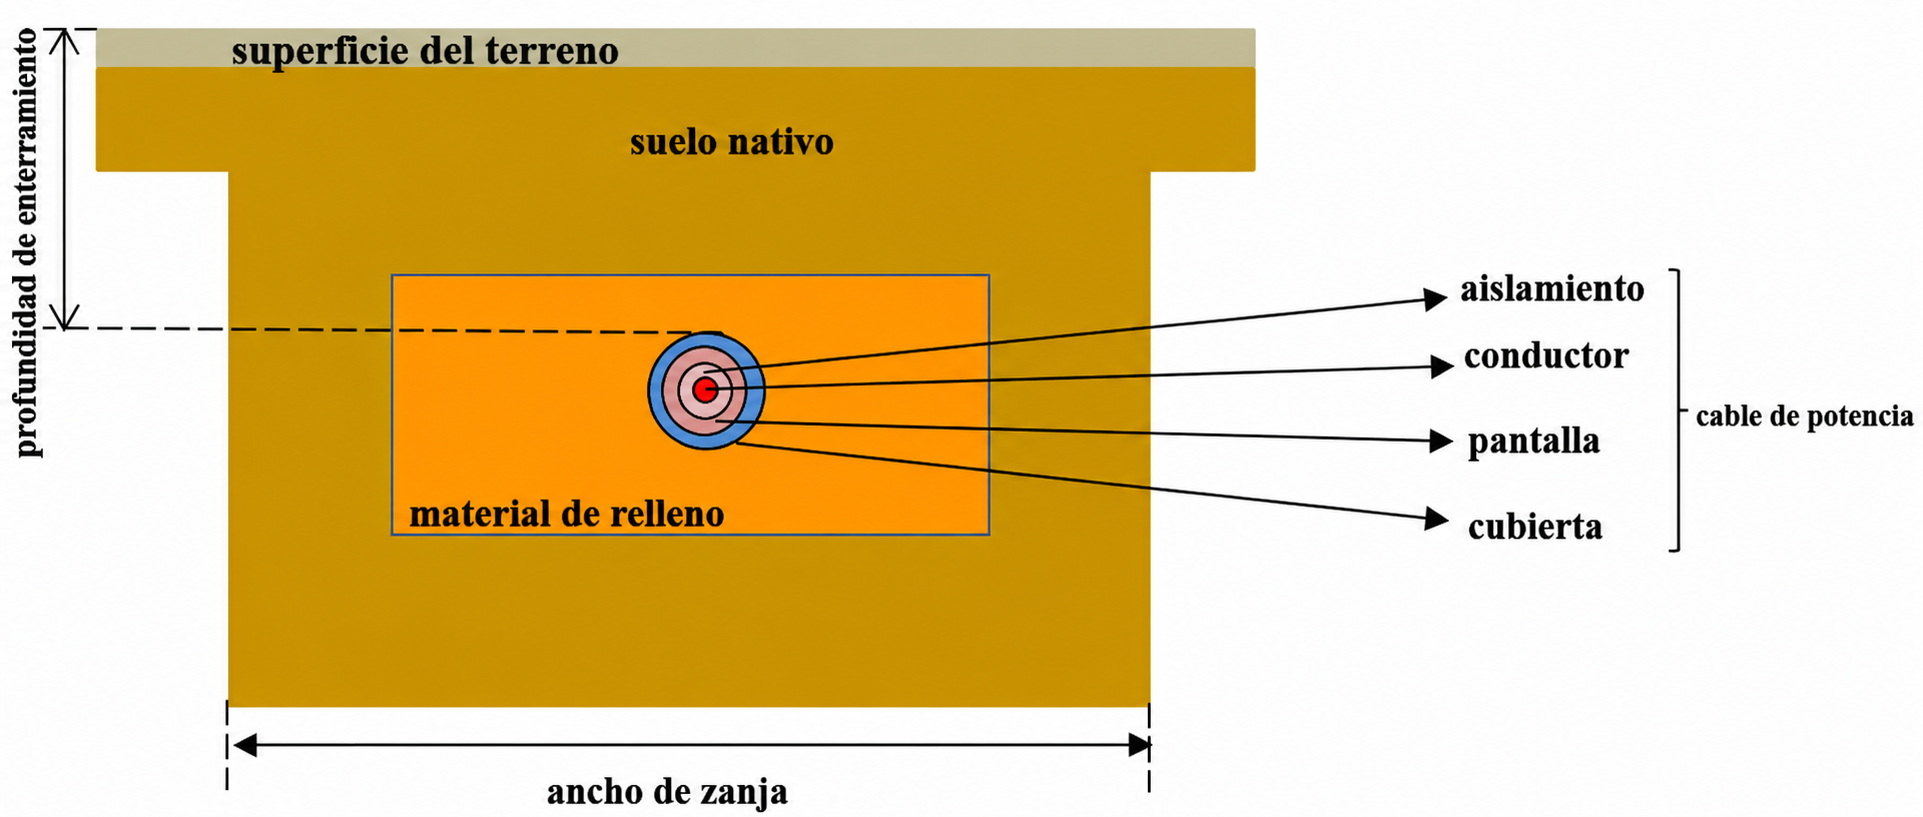
\includegraphics[width=1.08\linewidth,height=0.43\paperheight,keepaspectratio]{enescu_trench_xsection_es.png}}
\end{columns}

\vspace{-0.006\paperheight}
\centering
\begin{tikzpicture}[
  tax/.style={rounded corners=4pt,draw,text width=4.32cm,minimum height=0.80cm,
    align=left,inner sep=3pt,font=\fontsize{7.25}{8.25}\selectfont}]
\node[tax,fill=lightblue,draw=midblue] at (-4.65,0)
  {\textbf{Cable:} conductor, pantallas, aislamiento XLPE, capas metálicas y cubierta.};
\node[tax,fill=softorange,draw=orange] at (0,0)
  {\textbf{Instalación:} unipolar o tripolar; plana o trébol; profundidad y separación.};
\node[tax,fill=softgreen,draw=teal] at (4.65,0)
  {\textbf{Entorno:} material de asiento, relleno, suelo nativo, interfaces y humedad.};
\end{tikzpicture}
\vspace{0.002\paperheight}
{\centering\fontsize{7.35}{8.35}\selectfont\bfseries\textcolor{darkblue}{Ciclo de vida físico del objeto}\par}
\vspace{-0.002\paperheight}
\begin{tikzpicture}[>=Latex,
  life/.style={rounded corners=3pt,draw,text width=1.98cm,minimum height=0.51cm,
    align=center,inner sep=1.2pt,font=\fontsize{5.9}{6.7}\selectfont\bfseries},
  la/.style={-{Stealth[length=1.5mm]},line width=0.55pt,darkblue}]
\node[life,fill=lightblue,draw=midblue] (l1) at (-5.70,0) {Diseño físico};
\node[life,fill=lightblue,draw=midblue] (l2) at (-3.42,0) {Preparación del entorno};
\node[life,fill=lightblue,draw=midblue] (l3) at (-1.14,0) {Instalación};
\node[life,fill=softorange,draw=orange] (l4) at (1.14,0) {Operación};
\node[life,fill=softorange,draw=orange] (l5) at (3.42,0) {Evolución térmica};
\node[life,fill=softgreen,draw=teal] (l6) at (5.70,0) {Intervención o retiro};
\draw[la] (l1)--(l2); \draw[la] (l2)--(l3); \draw[la] (l3)--(l4);
\draw[la] (l4)--(l5); \draw[la] (l5)--(l6);
\end{tikzpicture}
\source[\fontsize{5.9}{6.8}\selectfont]{Estructura basada en \textcite{kim2025} e IEC 60502-2 \parencite{iec60502_2_2014}; sección de zanja adaptada de \textcite{enescu2021}.}
\note{Mostrar las dos escalas del objeto, resumir su taxonomía y cerrar con el ciclo de vida físico. La ampacidad pertenece al conjunto, no al cable aislado.}
\end{frame}

% 10 ------------------------------------------------------------------------
\begin{frame}{Instrumento para medir el objeto de estudio.}
\situacionsubyacente
\vspace{-0.004\paperheight}
\centering
\begin{tikzpicture}[>=Latex,
  src/.style={rounded corners=4pt,draw,text width=3.08cm,minimum height=1.62cm,
    align=left,inner sep=2.9pt,font=\fontsize{6.55}{7.45}\selectfont},
  proc/.style={rounded corners=3pt,draw=darkblue!65,text width=2.22cm,
    minimum height=0.68cm,align=center,inner sep=2.2pt,
    font=\fontsize{6.25}{7.1}\selectfont},
  flow/.style={-{Stealth[length=1.8mm]},line width=0.65pt,darkblue}]

\node[rounded corners=5pt,draw=midblue,fill=lightblue,text width=13.55cm,
  minimum height=0.82cm,align=left,inner sep=4.2pt,
  font=\fontsize{9.15}{10.4}\selectfont] at (0,2.45)
  {\textbf{No se empleará un sensor.} El instrumento es el protocolo documental y computacional que transforma referencias independientes en casos térmicos 2D trazables.};

\node[src,fill=lightblue,draw=midblue] at (-5.10,1.03)
  {\textbf{Solución manufacturada}\par Se prescribe $T(x,y)$ y se derivan $Q$, contornos e interfaces: referencia exacta del proyecto.};
\node[src,fill=warmgray,draw=textgray!60] at (-1.70,1.03)
  {\textbf{Analítica / normativa}\par Soluciones cerradas e IEC 60287 para casos simples y línea base de ampacidad.};
\node[src,fill=softgreen,draw=teal] at (1.70,1.03)
  {\textbf{FEM independiente}\par FEniCSx o FEM publicado con malla y convergencia; p. ej., COMSOL en Kim.};
\node[src,fill=softorange,draw=orange] at (5.10,1.03)
  {\textbf{Publicaciones y valores típicos}\par Khumalo, Arias, Atoccsa y Kim; más normas, fichas y literatura con trazabilidad.};

\node[font=\fontsize{8.2}{9.25}\selectfont\bfseries,text=darkblue] at (0,-0.10)
  {Cómo se obtiene y registra cada caso};
\node[proc,fill=warmgray] (p1) at (-5.20,-0.88)
  {\textbf{1. Localizar}\par DOI · PDF · repositorio};
\node[proc,fill=lightblue] (p2) at (-2.60,-0.88)
  {\textbf{2. Extraer}\par página · tabla · figura};
\node[proc,fill=softorange,draw=orange] (p3) at (0,-0.88)
  {\textbf{3. Normalizar}\par unidades · $k$ · supuestos};
\node[proc,fill=softgreen,draw=teal] (p4) at (2.60,-0.88)
  {\textbf{4. Parametrizar}\par dominio · capas · contornos};
\node[proc,fill=lightblue] (p5) at (5.20,-0.88)
  {\textbf{5. Registrar referencia}\par $T$, $\Tmax$, $\Imax$ · versión};
\draw[flow] (p1)--(p2); \draw[flow] (p2)--(p3); \draw[flow] (p3)--(p4); \draw[flow] (p4)--(p5);

\node[rounded corners=4pt,draw=unired,fill=softred,text width=13.55cm,
  minimum height=0.64cm,align=left,inner sep=3.2pt,
  font=\fontsize{7.55}{8.6}\selectfont] at (0,-1.98)
  {\textbf{Regla de trazabilidad:} cada dato conserva fuente, página/tabla/figura, unidad y supuesto. No habrá mediciones ni validación experimental en campo.};
\end{tikzpicture}
\source[\fontsize{5.8}{6.7}\selectfont]{Protocolo del plan; verificación según \textcite{cigre2025} e IEC 60287 \parencite{iec60287}; casos publicados: \textcite{khumalo2025}, \textcite{ariasVelasquez2023}, \textcite{atoccsa2024} y \textcite{kim2025}.}
\note{Explicar que el equivalente funcional del instrumento es el protocolo de extracción y parametrización. Distinguir las fuentes de referencia y señalar que no existe captura sensorial ni campaña de campo.}
\end{frame}

% 11 ------------------------------------------------------------------------
\begin{frame}{Objeto de estudio modelado}
\situacionsubyacente
\vspace{-0.004\paperheight}
\centering
\begin{tikzpicture}[x=1cm,y=1cm]
\node[rounded corners=5pt,draw=orange,fill=softorange,text width=13.55cm,
  minimum height=0.82cm,align=left,inner sep=4.2pt,
  font=\fontsize{9.1}{10.35}\selectfont] at (0,2.42)
  {\textbf{Representación formal del objeto real:} sección 2D definida por el dominio $\Omega$, regiones del cable, interfaces, $\kx$, fuente térmica $Q$ y condiciones de contorno.};

\begin{scope}[shift={(-4.65,0.42)}]
  \draw[rounded corners=4pt,draw=midblue,line width=0.7pt,fill=white] (-2.15,-0.96) rectangle (2.15,1.32);
  \node[font=\fontsize{8.0}{9.0}\selectfont\bfseries,text=darkblue] at (0,1.08) {H0 · Homogéneo equivalente};
  \fill[orange!28] (-1.68,-0.22) rectangle (1.68,0.68);
  \draw[textgray!55] (-1.68,0.68)--(1.68,0.68);
  \foreach \cx in {-0.55,0,0.55}{
    \fill[black!75] (\cx,0.05) circle (0.16);
    \fill[orange!85] (\cx,0.05) circle (0.095);
  }
  \node[font=\fontsize{6.4}{7.2}\selectfont\bfseries,text=orange!80!black] at (1.20,0.48) {$k_{\mathrm{eq}}$};
  \node[font=\fontsize{6.8}{7.7}\selectfont,align=center,text width=3.85cm] at (0,-0.65)
    {Un valor equivalente representa todo el entorno.};
\end{scope}

\begin{scope}[shift={(0,0.42)}]
  \draw[rounded corners=4pt,draw=orange,line width=0.7pt,fill=white] (-2.15,-0.96) rectangle (2.15,1.32);
  \node[font=\fontsize{8.0}{9.0}\selectfont\bfseries,text=orange!80!black] at (0,1.08) {H1 · Estratificado};
  \fill[orange!18] (-1.68,0.38) rectangle (1.68,0.68);
  \fill[orange!35] (-1.68,0.08) rectangle (1.68,0.38);
  \fill[orange!55] (-1.68,-0.22) rectangle (1.68,0.08);
  \draw[textgray!45] (-1.68,0.68)--(1.68,0.68);
  \foreach \cx in {-0.55,0,0.55}{
    \fill[black!75] (\cx,0.05) circle (0.16);
    \fill[orange!85] (\cx,0.05) circle (0.095);
  }
  \node[font=\fontsize{5.8}{6.5}\selectfont] at (1.38,0.53) {$k_1$};
  \node[font=\fontsize{5.8}{6.5}\selectfont] at (1.38,0.23) {$k_2$};
  \node[font=\fontsize{5.8}{6.5}\selectfont] at (1.38,-0.07) {$k_3$};
  \node[font=\fontsize{6.8}{7.7}\selectfont,align=center,text width=3.85cm] at (0,-0.65)
    {Estratos con conductividades y espesores distintos.};
\end{scope}

\begin{scope}[shift={(4.65,0.42)}]
  \draw[rounded corners=4pt,draw=teal,line width=0.7pt,fill=white] (-2.15,-0.96) rectangle (2.15,1.32);
  \node[font=\fontsize{8.0}{9.0}\selectfont\bfseries,text=teal!80!black] at (0,1.08) {H2 · Heterogeneidad localizada};
  \fill[orange!28] (-1.68,-0.22) rectangle (1.68,0.68);
  \fill[teal!28] (-1.14,-0.18) rectangle (0.98,0.37);
  \draw[teal!75,line width=0.5pt] (-1.14,-0.18) rectangle (0.98,0.37);
  \fill[softred] (1.27,0.42) circle (0.23);
  \draw[unired,line width=0.5pt] (1.27,0.42) circle (0.23);
  \foreach \cx in {-0.55,0,0.55}{
    \fill[black!75] (\cx,0.05) circle (0.16);
    \fill[orange!85] (\cx,0.05) circle (0.095);
  }
  \node[font=\fontsize{5.6}{6.3}\selectfont,text=teal!80!black] at (-0.75,0.52) {$k$ alta};
  \node[font=\fontsize{5.6}{6.3}\selectfont,text=unired] at (1.25,0.75) {$k$ baja};
  \node[font=\fontsize{6.8}{7.7}\selectfont,align=center,text width=3.85cm] at (0,-0.65)
    {Relleno conductor o zona seca de baja $k$ cerca del cable.};
\end{scope}

\node[rounded corners=4pt,draw=textgray!55,fill=warmgray,text width=13.55cm,
  minimum height=0.78cm,align=left,inner sep=3.8pt,
  font=\fontsize{7.75}{8.8}\selectfont] at (0,-1.46)
  {\textbf{Instanciación en el proyecto:} archivos parametrizados de dominio, capas del cable, posiciones, propiedades del suelo, contornos y escenarios; cada caso conserva referencia y versión.};
\end{tikzpicture}
\source[\fontsize{6.0}{6.9}\selectfont]{Modelo operativo y diseño factorial del plan; geometrías de referencia basadas en \textcite{enescu2021} y \textcite{kim2025}; estructura de archivos del proyecto.}
\note{Presentar los tres estados principales del objeto modelado. Aclarar que contraste, extensión y proximidad refinan H1 y H2, mientras $T(x,y)$, $\Tmax$ e $\Imax$ son respuestas calculadas, no el objeto real.}
\end{frame}

% 12 ------------------------------------------------------------------------
\begin{frame}{Problema Tecnológico: Artefacto PINN 2D}
\situaciontecnologica
\vspace{-0.003\paperheight}
\centering
\begin{tikzpicture}[>=Latex,
  core/.style={rounded corners=4pt,draw,text width=2.35cm,minimum height=1.00cm,
    align=center,inner sep=2.7pt,font=\fontsize{7.15}{8.15}\selectfont},
  op/.style={rounded corners=3pt,draw=darkblue!65,text width=1.27cm,
    minimum height=0.72cm,align=center,inner sep=1.6pt,
    font=\fontsize{5.35}{6.1}\selectfont},
  arr/.style={-{Stealth[length=2.0mm]},line width=0.7pt,darkblue},
  feedback/.style={-{Stealth[length=1.8mm]},line width=0.65pt,dashed,darkblue}]

\node[font=\fontsize{9.4}{10.5}\selectfont\bfseries,text=darkblue] at (-2.70,2.60)
  {Arquitectura y operación};
\node[core,fill=lightblue,draw=midblue] (inp) at (-5.55,1.48)
  {\textbf{Entradas físicas}\\$(x,y)$ · geometría · $\kx$\\$Q$ · contornos · interfaces · $I$};
\node[core,fill=softgreen,draw=teal] (pinn) at (-2.70,1.48)
  {\textbf{Red PINN (MLP)}\\aproxima el campo\\$T(x,y)$};
\node[core,fill=softorange,draw=orange] (temp) at (0.15,1.48)
  {\textbf{Respuesta térmica}\\$T(x,y)$ y $\Tmax$\\residuos y balance};
\draw[arr] (inp)--(pinn); \draw[arr] (pinn)--(temp);

\node[rounded corners=4pt,draw=orange,fill=softorange,text width=6.55cm,
  minimum height=0.58cm,align=center,inner sep=2.5pt,
  font=\fontsize{6.45}{7.35}\selectfont] (loss) at (-2.70,0.30)
  {\textbf{Entrenamiento:} diferenciación automática + pérdida $\mathcal L_{\mathrm{PDE}}+\mathcal L_{\mathrm{cont}}+\mathcal L_{\mathrm{int}}+\mathcal L_{\mathrm{ene}}$ $(+\mathcal L_{\mathrm{datos}}$ si existe referencia$)$};
\draw[arr] (temp.south) to[bend left=12] (loss.north east);
\draw[feedback] (loss.north)--(pinn.south);

\node[font=\fontsize{7.8}{8.8}\selectfont\bfseries,text=darkblue] at (-2.70,-0.42)
  {Modo de operación};
\node[op,fill=warmgray] (o1) at (-5.80,-1.03) {1. Parametrizar\\escenario};
\node[op,fill=lightblue] (o2) at (-4.25,-1.03) {2. Muestrear\\y entrenar};
\node[op,fill=softgreen,draw=teal] (o3) at (-2.70,-1.03) {3. Obtener\\$T$ y $\Tmax$};
\node[op,fill=softorange,draw=orange] (o4) at (-1.15,-1.03) {4. Iterar $I$\\hasta $T_{\mathrm{lim}}$};
\node[op,fill=warmgray] (o5) at (0.40,-1.03) {5. Verificar\\y registrar};
\draw[arr] (o1)--(o2); \draw[arr] (o2)--(o3); \draw[arr] (o3)--(o4); \draw[arr] (o4)--(o5);

\node[rounded corners=4pt,draw=textgray!55,fill=warmgray,text width=7.55cm,
  minimum height=0.58cm,align=left,inner sep=3pt,
  font=\fontsize{6.45}{7.35}\selectfont] at (-2.70,-1.93)
  {\textbf{Verificación:} soluciones analíticas o manufacturadas, FEM convergente y casos publicados; reporte de error, residuo, balance, robustez y trazabilidad.};

\node[rounded corners=5pt,draw=midblue,line width=0.8pt,fill=lightblue,
  text width=4.62cm,minimum height=5.05cm,align=left,inner sep=5pt,
  font=\fontsize{7.15}{8.15}\selectfont] at (4.12,0.18)
  {{\fontsize{9.0}{10.1}\selectfont\bfseries\textcolor{darkblue}{Características del artefacto}}\par\vspace{1.2mm}
   \textbf{Qué se construirá:} modelo lógico y prototipo computacional PINN 2D para analizar el arreglo cable--entorno térmico.\par\vspace{1.0mm}
   \textbf{Naturaleza:} software científico; el hardware de cómputo es plataforma de ejecución, no parte del artefacto. No requiere comunicaciones.\par\vspace{1.0mm}
   \textbf{Problema de ML:} regresión informada por física del campo continuo $T(x,y)$; no clasificación, pronóstico ni asociación.\par\vspace{1.0mm}
   \textbf{Integra:} PDE de calor, contornos, interfaces, $\kx$, búsqueda de $\Imax$, verificación y trazabilidad.\par\vspace{1.0mm}
   \textbf{Alcance:} régimen estacionario 2D; evaluación mediante verificación computacional, sin validación experimental de campo.};
\end{tikzpicture}
\source[\fontsize{6.3}{7.2}\selectfont]{Arquitectura lógica del plan; formulación PINN basada en \textcite{raissi2019}; evaluación DSR basada en \textcite{peffers2007} y \textcite{gregor2013}.}
\note{Definir el artefacto como software científico y no como hardware. Explicar que la tarea de ML es regresión de un campo continuo y recorrer la arquitectura y el modo de operación hasta obtener y verificar la ampacidad.}
\end{frame}

\section{Problemas y objetivos}

% 13 ------------------------------------------------------------------------
\begin{frame}{Planteamiento del Problema Tecnológico}
\situaciontecnologica
\vspace{-0.004\paperheight}
\centering
\begin{tikzpicture}[>=Latex,
  pg/.style={rounded corners=5pt,draw,text width=13.35cm,align=left,
    inner sep=4.2pt,font=\fontsize{7.85}{8.95}\selectfont},
  a/.style={-{Stealth[length=2.1mm]},line width=0.80pt,darkblue,shorten <=1pt,shorten >=1pt}]
\node[font=\fontsize{10.3}{11.5}\selectfont\bfseries,text=darkblue] at (0,2.73)
  {Problema General};
\node[pg,fill=lightblue,draw=midblue,minimum height=1.20cm] (g1) at (0,1.68)
  {En el arreglo de cables--entorno térmico, la heterogeneidad espacial del suelo, el asiento y los rellenos puede modificar $T(x,y)$, $\Tmax$ e $\Imax$ respecto de una representación homogénea equivalente. Sin embargo, resulta difícil cuantificar esas diferencias de forma reproducible y establecer cuándo son relevantes para las decisiones de diseño y operación.};
\node[pg,fill=warmgray,draw=textgray!55,minimum height=1.04cm] (g2) at (0,0.05)
  {Las representaciones homogéneas equivalentes son rápidas, aunque no describen de forma explícita la conductividad variable $\kx$; los modelos FEM sí pueden representarla, pero exigen construir, mallar y verificar cada escenario.};
\node[pg,fill=softorange,draw=orange,minimum height=1.02cm] (g3) at (0,-1.43)
  {En consecuencia, persiste la necesidad de una formulación computacional verificada y trazable que represente $\kx$, estime el campo térmico y documente la exactitud, la consistencia física y la robustez del análisis.};
\draw[a] (g1)--(g2); \draw[a] (g2)--(g3);
\node[rounded corners=4pt,draw=unired,fill=softred,text width=13.35cm,
  minimum height=0.56cm,align=left,inner sep=3.2pt,
  font=\fontsize{6.9}{7.85}\selectfont] at (0,-2.47)
  {\textbf{Delimitación tecnológica:} el problema se relaciona exclusivamente con el artefacto computacional que se construirá y evaluará; no plantea resolver directamente la planificación ni la operación del sistema eléctrico.};
\end{tikzpicture}
\source[\fontsize{6.1}{7.0}\selectfont]{Formulación sustentada en \textcite{enescu2021}, IEC 60287--60853 \parencite{iec60287,iec60853}, \textcite{cigre2025} y \textcite{raissi2019}.}
\note{Leer el problema como situación declarativa. Distinguir el fenómeno físico, las limitaciones de las representaciones existentes y la necesidad tecnológica centrada en el artefacto.}
\end{frame}

% 14 ------------------------------------------------------------------------
\begin{frame}{Problemas específicos 1/2}
\vspace{-0.014\paperheight}
\centering
\begin{tikzpicture}[>=Latex,
  ins/.style={rounded corners=3pt,draw=textgray!45,fill=white,text width=3.95cm,
    minimum height=0.64cm,align=center,inner sep=2.5pt,
    font=\fontsize{6.2}{7.05}\selectfont},
  pe/.style={rounded corners=5pt,draw,text width=4.02cm,minimum height=2.55cm,
    align=left,inner sep=4pt,font=\fontsize{7.15}{8.1}\selectfont},
  a/.style={-{Stealth[length=2.2mm]},line width=0.82pt,darkblue,shorten <=1pt,shorten >=1pt},
  d/.style={font=\fontsize{6.1}{6.9}\selectfont\bfseries,fill=white,inner sep=1.2pt,text=darkblue,yshift=2pt}]
\node[ins] (i1) at (-4.78,2.18) {Cable multicapa, interfaces, fuentes, contornos y $\kx$};
\node[ins] (i2) at (0,2.18) {Soluciones analíticas o manufacturadas, FEM y casos publicados};
\node[ins] (i3) at (4.78,2.18) {Contraste, patrón, extensión y proximidad};
\node[pe,fill=warmgray,draw=textgray!60] (pe1) at (-4.78,0.35)
  {\textbf{PE1.} La representación física requerida por el artefacto no está formalizada en términos de entradas, requisitos funcionales y criterios de calidad que ordenen el cable multicapa, las interfaces, las fuentes, los contornos y $\kx$ en escenarios heterogéneos.};
\node[pe,fill=lightblue,draw=midblue] (pe2) at (0,0.35)
  {\textbf{PE2.} No se dispone de un paquete reproducible de soluciones analíticas o manufacturadas, referencias FEM con convergencia y casos publicados que permita construir y verificar el artefacto dentro del dominio delimitado.};
\node[pe,fill=softgreen,draw=teal] (pe3) at (4.78,0.35)
  {\textbf{PE3.} No se ha cuantificado de forma trazable cómo el contraste, el patrón, la extensión y la proximidad de las heterogeneidades modifican $\Tmax$, el campo $T(x,y)$ y la localización del punto caliente.};
\draw[a] (i1)--(pe1); \draw[a] (i2)--(pe2); \draw[a] (i3)--(pe3);
\draw[a] (pe1)--node[d,above]{D1}(pe2); \draw[a] (pe2)--node[d,above]{D2}(pe3);
\node[rounded corners=4pt,draw=darkblue,fill=lightblue,text width=13.20cm,
  minimum height=0.62cm,align=center,inner sep=3pt,
  font=\fontsize{7.3}{8.25}\selectfont\bfseries] at (0,-1.78)
  {Especificar la representación $\rightarrow$ integrar referencias de verificación $\rightarrow$ cuantificar escenarios heterogéneos};
\end{tikzpicture}
\source[\fontsize{6.0}{6.9}\selectfont]{Problemas y articulación sustentados en verificación DSR \parencite{peffers2007,gregor2013} y referencias térmicas \parencite{enescu2021,cigre2025}.}
\note{Presentar PE1, PE2 y PE3 como situaciones del artefacto. Los insumos superiores y las flechas D1--D2 reproducen la lógica de articulación del plan.}
\end{frame}

% 15 ------------------------------------------------------------------------
\begin{frame}{Problemas específicos 2/2}
\vspace{-0.014\paperheight}
\centering
\begin{tikzpicture}[>=Latex,
  ins/.style={rounded corners=3pt,draw=textgray!45,fill=white,text width=6.10cm,
    minimum height=0.58cm,align=center,inner sep=2.5pt,
    font=\fontsize{6.3}{7.1}\selectfont},
  pe/.style={rounded corners=5pt,draw,text width=6.12cm,minimum height=2.10cm,
    align=left,inner sep=4pt,font=\fontsize{7.45}{8.45}\selectfont},
  mini/.style={rounded corners=3pt,draw,text width=1.82cm,minimum height=0.72cm,
    align=center,inner sep=1.6pt,font=\fontsize{5.35}{6.05}\selectfont\bfseries},
  a/.style={-{Stealth[length=2.1mm]},line width=0.78pt,darkblue,shorten <=1pt,shorten >=1pt},
  d/.style={font=\fontsize{5.9}{6.6}\selectfont\bfseries,fill=white,inner sep=1.1pt,text=darkblue,yshift=2pt}]
\node[ins] (i4) at (-3.48,2.52) {Representaciones homogénea equivalente y heterogénea 2D verificada};
\node[ins] (i5) at (3.48,2.52) {Evidencia y criterios de evaluación producidos por el artefacto};
\node[pe,fill=softorange,draw=orange] (pe4) at (-3.48,0.95)
  {\textbf{PE4.} No se han identificado las condiciones que producen la mayor discrepancia de ampacidad entre una representación 2D heterogénea verificada y una representación homogénea equivalente.};
\node[pe,fill=softred,draw=unired] (pe5) at (3.48,0.95)
  {\textbf{PE5.} No se ha sistematizado, a partir de la evidencia del artefacto, un procedimiento reproducible ni principios de diseño para problemas térmicos 2D multimateriales de cables enterrados.};
\draw[a] (i4)--(pe4); \draw[a] (i5)--(pe5);
\draw[a] (pe4)--node[d,above]{D4}(pe5);

\node[font=\fontsize{7.7}{8.7}\selectfont\bfseries,text=darkblue] at (0,-0.45)
  {Articulación secuencial del plan};
\node[mini,fill=warmgray] (m1) at (-5.75,-1.32) {PE1\\Representación};
\node[mini,fill=lightblue,draw=midblue] (m2) at (-3.45,-1.32) {PE2\\Referencias};
\node[mini,fill=softgreen,draw=teal] (m3) at (-1.15,-1.32) {PE3\\Escenarios};
\node[mini,fill=softorange,draw=orange] (m4) at (1.15,-1.32) {PE4\\Ampacidad};
\node[mini,fill=softred,draw=unired] (m5) at (3.45,-1.32) {PE5\\Procedimiento};
\node[mini,fill=lightblue,draw=darkblue] (res) at (5.75,-1.32) {Resultado lógico\\objetivos};
\draw[a] (m1)--node[d,above]{D1}(m2); \draw[a] (m2)--node[d,above]{D2}(m3);
\draw[a] (m3)--node[d,above]{D3}(m4); \draw[a] (m4)--node[d,above]{D4}(m5);
\draw[a] (m5)--(res);
\node[rounded corners=4pt,draw=textgray!55,fill=warmgray,text width=13.20cm,
  minimum height=0.58cm,align=center,inner sep=3pt,
  font=\fontsize{6.65}{7.55}\selectfont] at (0,-2.20)
  {Cada situación recibe evidencia del artefacto y produce una definición o resultado necesario para abordar la siguiente.};
\end{tikzpicture}
\source[\fontsize{6.0}{6.9}\selectfont]{Articulación DSR del plan \parencite{peffers2007,gregor2013}; comparación térmica y verificación según \textcite{cigre2025}.}
\note{Cerrar PE4 y PE5 y recorrer la secuencia completa. El plan vigente formula cinco problemas específicos; no inventar un PE6 sin modificar previamente el documento matriz.}
\end{frame}

% 16 ------------------------------------------------------------------------
\begin{frame}{Objetivo General}
\vspace{-0.018\paperheight}
\centering
\begin{tikzpicture}[>=Latex,
 b/.style={rounded corners=5pt,draw,align=center,text width=3.75cm,
   minimum height=1.50cm,font=\fontsize{7.60}{8.70}\selectfont,inner sep=4pt},
 a/.style={-{Stealth[length=2.3mm]},line width=0.85pt,darkblue}]
\node[rounded corners=5pt,draw=teal,fill=softgreen,text width=13.35cm,
  minimum height=1.30cm,align=left,inner sep=5pt,
  font=\fontsize{9.2}{10.55}\selectfont] at (0,2.20)
  {\textbf{Objetivo general:} Diseñar y evaluar un artefacto computacional basado en una red neuronal informada por física (PINN) que represente el arreglo de cables--entorno térmico, estime el campo de temperaturas $T(x,y)$, la temperatura máxima del dominio $\Tmax$ y la ampacidad $\Imax$, cuantificar el efecto de la heterogeneidad térmica espacial y documentar su exactitud, consistencia física, robustez y reproducibilidad.};
\node[b,fill=lightblue,draw=midblue] (i) at (-4.70,0.15)
  {\textbf{Insumo inicial}\\Cable, geometría, fuentes $Q$, contornos, interfaces, $\kx$ y casos de referencia};
\node[b,fill=softgreen,draw=teal,text width=4.10cm] (o) at (0,0.15)
  {\textbf{Intervención investigada}\\Modelo y prototipo computacional PINN 2D especificado, construido y evaluado};
\node[b,fill=softorange,draw=orange] (r) at (4.70,0.15)
  {\textbf{Variables dependientes y medidas}\\$T(x,y)$, $\Tmax$, $\Imax$; error, balance, robustez y reproducibilidad};
\draw[a] (i)--(o); \draw[a] (o)--(r);
\node[rounded corners=4pt,draw=unired,fill=softred,text width=13.20cm,
  minimum height=0.58cm,align=center,inner sep=3pt,
  font=\fontsize{7.15}{8.15}\selectfont] at (0,-1.25)
  {El objetivo se relaciona con la construcción y evaluación del artefacto; programar, entrenar o ejecutar casos son actividades, no el objetivo de investigación.};
\end{tikzpicture}
\source[\fontsize{6.1}{7.0}\selectfont]{Objetivo y productos sustentados en DSR \parencite{peffers2007,gregor2013}; verificación térmica según \textcite{cigre2025} y formulación PINN de \textcite{raissi2019}.}
\note{Leer literalmente el objetivo general. Luego identificar el insumo inicial, la intervención y las variables dependientes o medidas de desempeño del artefacto.}
\end{frame}

% 17 ------------------------------------------------------------------------
\begin{frame}{Objetivos Específicos 1/2}
\vspace{-0.014\paperheight}
\centering
\begin{tikzpicture}[>=Latex,
  ins/.style={rounded corners=3pt,draw=textgray!45,fill=white,text width=3.95cm,
    minimum height=0.62cm,align=center,inner sep=2.4pt,
    font=\fontsize{6.05}{6.85}\selectfont},
  oe/.style={rounded corners=5pt,draw,text width=4.02cm,minimum height=3.25cm,
    align=left,inner sep=4pt,font=\fontsize{6.65}{7.55}\selectfont},
  a/.style={-{Stealth[length=2.2mm]},line width=0.82pt,darkblue,shorten <=1pt,shorten >=1pt},
  d/.style={font=\fontsize{6.0}{6.8}\selectfont\bfseries,fill=white,inner sep=1.2pt,text=darkblue,yshift=2pt}]
\node[ins] (i1) at (-4.78,2.48) {Cable, geometría, fuentes, contornos, interfaces y $\kx$};
\node[ins] (i2) at (0,2.48) {Soluciones analíticas, manufacturadas, FEM y publicadas};
\node[ins] (i3) at (4.78,2.48) {Contraste, patrón, extensión y proximidad};
\node[oe,fill=warmgray,draw=textgray!60] (oe1) at (-4.78,0.25)
  {\textbf{OE1.} Especificar las entradas físicas, requisitos funcionales y criterios de calidad del artefacto para representar el arreglo de cables--entorno térmico, incluyendo dominios multicapa, fuentes térmicas, condiciones de contorno, interfaces y conductividad térmica espacialmente variable $\kx$.\par\vspace{0.8mm}\textbf{Producto:} documento de requisitos, catálogo de materiales y geometrías, ficha de supuestos y matriz requisito--prueba.};
\node[oe,fill=lightblue,draw=midblue] (oe2) at (0,0.25)
  {\textbf{OE2.} Construir y verificar el artefacto mediante soluciones analíticas o manufacturadas, benchmarks FEM con convergencia y casos publicados, evaluando su exactitud, consistencia física y robustez entre ejecuciones.\par\vspace{0.8mm}\textbf{Producto:} base de benchmarks, casos manufacturados, referencias FEM convergentes e informe de verificación.};
\node[oe,fill=softgreen,draw=teal] (oe3) at (4.78,0.25)
  {\textbf{OE3.} Evaluar escenarios controlados de contraste, patrón, extensión y proximidad de heterogeneidades del suelo y los rellenos para obtener cambios en $\Tmax$, el campo de temperatura $T(x,y)$ y la localización del punto caliente.\par\vspace{0.8mm}\textbf{Producto:} mapas de $\kx$ y $T(x,y)$, resultados de sensibilidad y límites del artefacto.};
\draw[a] (i1)--(oe1); \draw[a] (i2)--(oe2); \draw[a] (i3)--(oe3);
\draw[a] (oe1)--node[d,above]{D1}(oe2); \draw[a] (oe2)--node[d,above]{D2}(oe3);
\end{tikzpicture}
\source[\fontsize{6.0}{6.9}\selectfont]{Objetivos, entradas y productos articulados mediante DSR \parencite{peffers2007,gregor2013}; referencias de verificación según \textcite{cigre2025}.}
\note{Cada OE es un hito. Presentar la entrada superior, leer literalmente el objetivo y cerrar con el producto medible que alimenta al objetivo siguiente.}
\end{frame}

% 18 ------------------------------------------------------------------------
\begin{frame}{Objetivos Específicos 2/2}
\vspace{-0.014\paperheight}
\centering
\begin{tikzpicture}[>=Latex,
  ins/.style={rounded corners=3pt,draw=textgray!45,fill=white,text width=6.08cm,
    minimum height=0.58cm,align=center,inner sep=2.4pt,
    font=\fontsize{6.2}{7.0}\selectfont},
  oe/.style={rounded corners=5pt,draw,text width=6.10cm,minimum height=2.55cm,
    align=left,inner sep=4pt,font=\fontsize{6.85}{7.85}\selectfont},
  mini/.style={rounded corners=3pt,draw,text width=1.82cm,minimum height=0.72cm,
    align=center,inner sep=1.6pt,font=\fontsize{5.25}{5.95}\selectfont\bfseries},
  a/.style={-{Stealth[length=2.1mm]},line width=0.78pt,darkblue,shorten <=1pt,shorten >=1pt},
  d/.style={font=\fontsize{5.8}{6.5}\selectfont\bfseries,fill=white,inner sep=1.1pt,text=darkblue,yshift=2pt}]
\node[ins] (i4) at (-3.48,2.75) {Escenarios heterogéneos y homogéneos equivalentes};
\node[ins] (i5) at (3.48,2.75) {Evidencia, métricas y límites de validez};
\node[oe,fill=softorange,draw=orange] (oe4) at (-3.48,0.95)
  {\textbf{OE4.} Comparar la ampacidad obtenida con representación 2D heterogénea frente a escenarios homogéneos equivalentes e identificar las condiciones de entrada que generan mayor discrepancia.\par\vspace{0.8mm}\textbf{Producto:} rutina de búsqueda de $\Imax$, tabla de cambios de ampacidad, escenarios críticos y comparación heterogéneo--homogéneo.};
\node[oe,fill=softred,draw=unired] (oe5) at (3.48,0.95)
  {\textbf{OE5.} Formular, a partir de los resultados del artefacto, principios de diseño y un procedimiento reproducible para aplicar y evaluar PINN en problemas térmicos multimateriales de cables enterrados.\par\vspace{0.8mm}\textbf{Producto:} repositorio, bitácora de versiones, guía de reproducción, principios de diseño e informe final DSR.};
\draw[a] (i4)--(oe4); \draw[a] (i5)--(oe5);
\draw[a] (oe4)--node[d,above]{D4}(oe5);
\node[font=\fontsize{7.6}{8.6}\selectfont\bfseries,text=darkblue] at (0,-0.60)
  {Articulación de objetivos y productos};
\node[mini,fill=warmgray] (m1) at (-5.75,-1.42) {OE1\\Requisitos};
\node[mini,fill=lightblue,draw=midblue] (m2) at (-3.45,-1.42) {OE2\\Verificación};
\node[mini,fill=softgreen,draw=teal] (m3) at (-1.15,-1.42) {OE3\\Escenarios};
\node[mini,fill=softorange,draw=orange] (m4) at (1.15,-1.42) {OE4\\Ampacidad};
\node[mini,fill=softred,draw=unired] (m5) at (3.45,-1.42) {OE5\\Procedimiento};
\node[mini,fill=lightblue,draw=darkblue] (res) at (5.75,-1.42) {Artefacto evaluado\\y reproducible};
\draw[a] (m1)--node[d,above]{D1}(m2); \draw[a] (m2)--node[d,above]{D2}(m3);
\draw[a] (m3)--node[d,above]{D3}(m4); \draw[a] (m4)--node[d,above]{D4}(m5);
\draw[a] (m5)--(res);
\node[rounded corners=4pt,draw=textgray!55,fill=warmgray,text width=13.20cm,
  minimum height=0.55cm,align=center,inner sep=2.8pt,
  font=\fontsize{6.45}{7.35}\selectfont] at (0,-2.23)
  {Cada OE genera un producto medible que constituye la entrada o evidencia necesaria para el siguiente hito.};
\end{tikzpicture}
\source[\fontsize{6.0}{6.9}\selectfont]{Articulación secuencial de objetivos y productos bajo DSR \parencite{peffers2007,gregor2013}; criterios técnicos según \textcite{cigre2025}.}
\note{Presentar OE4 y OE5 y recorrer la articulación completa. Aclarar que el plan vigente formula cinco objetivos específicos.}
\end{frame}

\section{Variables y método}

% 19 ------------------------------------------------------------------------
\begin{frame}{Variables independientes 1/2}
\centering
\begin{tikzpicture}[
 card/.style={rounded corners=4pt,draw,text width=2.55cm,minimum height=1.22cm,align=center,inner sep=3.5pt,font=\fontsize{7.2}{8.6}\selectfont},
 main/.style={rounded corners=5pt,draw=darkblue,fill=lightblue,text width=12.15cm,minimum height=0.78cm,align=center,inner sep=4pt,font=\fontsize{8.8}{10.3}\selectfont}]
\node[main] (vi) at (0,2.25) {\textbf{Variable independiente principal: conductividad térmica espacialmente variable $\kx$.}\\
\textbf{Intervención controlada:} el investigador configura su mapa en el suelo, el asiento o el relleno para construir escenarios comparables.};

\node[card,fill=softgreen,draw=teal] (p) at (-4.42,0.25) {\textcolor{teal}{\fontsize{9.0}{10.3}\selectfont\bfseries Patrón $P$}\\[0.7mm]
estratificado · inclusión de baja $k$ · relleno de alta $k$ · zona seca};
\node[card,fill=lightblue,draw=midblue] (c) at (-1.48,0.25) {\textcolor{darkblue}{\fontsize{9.0}{10.3}\selectfont\bfseries Contraste $C_k$}\\[0.7mm]
bajo · medio · alto\\magnitud fijada en el piloto};
\node[card,fill=softorange,draw=orange] (e) at (1.48,0.25) {\textcolor{orange}{\fontsize{9.0}{10.3}\selectfont\bfseries Extensión $f_h$}\\[0.7mm]
pequeña · media · grande\\tamaño normalizado};
\node[card,fill=softred,draw=unired] (d) at (4.42,0.25) {\textcolor{unired}{\fontsize{9.0}{10.3}\selectfont\bfseries Proximidad $d_h/D$}\\[0.7mm]
cercana · media · lejana\\respecto del conductor};

\node[rounded corners=4pt,draw=textgray!45,fill=warmgray,text width=12.15cm,minimum height=0.68cm,align=center,inner sep=3.5pt,font=\fontsize{8.0}{9.4}\selectfont] at (0,-1.30)
{\textbf{Representación de comparación $R$:} heterogénea explícita · homogénea equivalente · homogénea conservadora · homogénea optimista.};
\node[rounded corners=4pt,draw=teal,fill=softgreen,text width=12.15cm,minimum height=0.68cm,align=center,inner sep=3.5pt,font=\fontsize{7.7}{9.1}\selectfont] at (0,-2.30)
{Los estados se combinan en un diseño factorial de escenarios numéricos; cada caso heterogéneo se compara con su referencia homogénea manteniendo constantes las demás condiciones.};
\end{tikzpicture}
\source[\fontsize{6.4}{7.3}\selectfont]{Operacionalización y diseño factorial del estudio; heterogeneidad térmica documentada por \textcite{enescu2021}, \textcite{khumalo2025} y \textcite{kim2025}.}
\note{Tiempo sugerido: 60 s. Precisar que la intervención controlada es la configuración espacial de k(x,y), no un hiperparámetro de entrenamiento.}
\end{frame}

% 20 ------------------------------------------------------------------------
\begin{frame}{Variables independientes 2/2}
\centering
\begin{tikzpicture}[
 card/.style={rounded corners=5pt,draw,text width=5.35cm,minimum height=1.48cm,align=left,inner sep=5pt,font=\fontsize{8.3}{9.8}\selectfont}]
\node[card,fill=softgreen,draw=teal] at (-3.15,1.65) {{\color{teal}\fontsize{10.5}{11.8}\selectfont\bfseries VI: factores modificados}\\[0.8mm]
Mapa $\kx$ y patrón $P$ · contraste $C_k$ · extensión $f_h$ · proximidad $d_h/D$ · representación $R$.\\[0.5mm]
Se configuran deliberadamente para contrastar su efecto.};

\node[card,fill=lightblue,draw=darkblue] at (3.15,1.65) {{\color{darkblue}\fontsize{10.5}{11.8}\selectfont\bfseries Controles pareados}\\[0.8mm]
Geometría y disposición · pérdidas $I^2R$ · contornos y dominio · $T_{\mathrm{amb}}$ y carga.\\[0.5mm]
La configuración numérica se congela después del piloto.};

\node[card,fill=softorange,draw=orange] at (-3.15,-1.05) {{\color{orange}\fontsize{10.5}{11.8}\selectfont\bfseries Metadatos registrados}\\[0.8mm]
Semilla y convergencia · tolerancia FEM · incertidumbre documental · versión del código · tiempo, memoria y hardware.\\[0.5mm]
Se registran para interpretar la evidencia; no se les atribuye el efecto físico.};

\node[card,fill=softred,draw=unired] at (3.15,-1.05) {{\color{unired}\fontsize{10.5}{11.8}\selectfont\bfseries No son VI del estudio}\\[0.8mm]
Épocas, lote, capas, neuronas, optimizador y tasa; tampoco las coordenadas $(x,y)$ ni las entradas mantenidas fijas.\\[0.5mm]
Son hiperparámetros o características del modelo.};

\node[rounded corners=4pt,draw=unired,fill=softred,text width=12.10cm,minimum height=0.68cm,align=center,inner sep=3.5pt,font=\fontsize{7.9}{9.3}\selectfont] at (0,-2.90)
{\textbf{Regla de interpretación:} que una magnitud ingrese a la PINN no la convierte en variable independiente; solo lo es si se modifica deliberadamente para contrastar su efecto.};
\end{tikzpicture}
\source[\fontsize{6.3}{7.2}\selectfont]{Operacionalización del estudio y comparaciones pareadas; verificación de herramientas de ampacidad según \textcite{cigre2025} y trazabilidad DSR según \textcite{gregor2013}.}
\note{Tiempo sugerido: 55 s. Distinguir factores, controles, condiciones registradas e hiperparámetros. La arquitectura queda fijada después del piloto.}
\end{frame}

% 21 ------------------------------------------------------------------------
\begin{frame}{Variables dependientes 1/2}
\centering
\begin{tikzpicture}[
 head/.style={rounded corners=4pt,draw=darkblue,fill=lightblue,text width=11.25cm,minimum height=0.72cm,align=center,inner sep=4pt,font=\fontsize{9.2}{10.8}\selectfont},
 tag/.style={rounded corners=4pt,draw,text width=1.02cm,minimum height=1.18cm,align=center,inner sep=3pt,font=\fontsize{10.2}{11.5}\selectfont\bfseries},
 body/.style={rounded corners=4pt,draw,text width=5.45cm,minimum height=1.18cm,align=left,inner sep=4pt,font=\fontsize{8.2}{9.7}\selectfont},
 met/.style={rounded corners=4pt,draw,text width=4.38cm,minimum height=1.18cm,align=left,inner sep=4pt,font=\fontsize{8.0}{9.5}\selectfont}]
\node[head] at (0,2.18) {\textbf{VD del artefacto: calidad técnica} = exactitud + consistencia física + robustez + reproducibilidad. Se observa mediante los resultados de cada objetivo.};

\node[tag,fill=warmgray,draw=textgray!55] at (-5.52,0.83) {OE1};
\node[body,fill=warmgray,draw=textgray!55] at (-1.82,0.83) {\textbf{Calidad de la especificación.} Cobertura de requisitos y trazabilidad requisito--prueba.};
\node[met,fill=white,draw=textgray!45] at (3.60,0.83) {$C_R=100\,n_{\mathrm{req\text{-}prueba}}/n_{\mathrm{req}}$\\$C_R\in[0,100]\pct$; meta: requisitos críticos cubiertos.};

\node[tag,fill=lightblue,draw=midblue] at (-5.52,-0.52) {OE2};
\node[body,fill=lightblue,draw=midblue] at (-1.82,-0.52) {\textbf{Exactitud, física y robustez.} Error de $\Tmax$, NRMSE, residuo, balance energético y variabilidad entre semillas.};
\node[met,fill=white,draw=midblue] at (3.60,-0.52) {$e_{T_{\max},\mathrm{PINN}}\leq5\pct$; NRMSE $\leq5\pct$; desequilibrio $\leq2\pct$. Umbrales iniciales.};

\node[tag,fill=softgreen,draw=teal] at (-5.52,-1.87) {OE3};
\node[body,fill=softgreen,draw=teal] at (-1.82,-1.87) {\textbf{Respuesta térmica.} $T(x,y)$, $\Tmax$, $\Delta\Tmax$ y localización del punto caliente $(x_h,y_h)$.};
\node[met,fill=white,draw=teal] at (3.60,-1.87) {$\Delta\Tmax=T_{\max}^{\mathrm{het}}-T_{\max}^{\mathrm{hom}}\in\mathbb{R}\,{}^\circ$C.\\Operación admisible: $\Tmax\leq T_{\mathrm{lim}}$; $(x_h,y_h)\in\Omega_c$.};
\end{tikzpicture}
\source[\fontsize{6.2}{7.1}\selectfont]{Correspondencia OE--indicadores del plan; criterios de verificación térmica según \textcite{cigre2025} y evaluación DSR según \textcite{gregor2013}.}
\note{Tiempo sugerido: 65 s. Indicar qué resultado se observa en OE1--OE3, su forma de cálculo y los criterios iniciales de aceptación.}
\end{frame}

% 22 ------------------------------------------------------------------------
\begin{frame}{Variables dependientes 2/2}
\centering
\begin{tikzpicture}[
 tag/.style={rounded corners=5pt,draw,text width=1.02cm,minimum height=1.18cm,align=center,inner sep=3pt,font=\fontsize{10.2}{11.5}\selectfont\bfseries},
 card/.style={rounded corners=5pt,draw,text width=4.03cm,minimum height=2.22cm,align=left,inner sep=6pt,font=\fontsize{8.25}{9.8}\selectfont},
 formula/.style={rounded corners=4pt,draw=textgray!45,fill=warmgray,text width=5.30cm,minimum height=0.98cm,align=center,inner sep=4pt,font=\fontsize{9.2}{11.0}\selectfont}]
\node[tag,fill=softorange,draw=orange,text=orange] at (-5.40,1.15) {OE4};
\node[card,fill=softorange,draw=orange] at (-2.46,1.15) {{\color{orange}\fontsize{10.2}{11.5}\selectfont\bfseries Resultado operativo}\\[1.0mm]
\textbf{Ampacidad $\Imax$:} corriente máxima compatible con $T_{\mathrm{lim}}$.\\[1mm]
\textbf{Indicadores:} $\Imax>0$ A; $\Delta I\in\mathbb{R}\pct$; margen térmico $T_{\mathrm{lim}}-\Tmax$ en $^\circ$C.};
\node[tag,fill=softred,draw=unired,text=unired] at (0.65,1.15) {OE5};
\node[card,fill=softred,draw=unired] at (3.59,1.15) {{\color{unired}\fontsize{10.2}{11.5}\selectfont\bfseries Reproducibilidad y aporte}\\[1.0mm]
\textbf{Resultados:} casos aceptados reproducidos, cobertura documental, límites de validez y principios de diseño.\\[1mm]
\textbf{Indicador:} $C_{\mathrm{rep}}\in[0,100]\pct$; meta: casos aceptados reproducibles.};

\node[formula] at (-3.02,-1.18) {$\displaystyle
\begin{gathered}
\Tmax(I)=\max_{(x,y)\in\Omega_c}T(x,y;I),\\[-0.4mm]
\Imax=\max\!\left\{I:\Tmax(I)\leq T_{\mathrm{lim}}\right\}
\end{gathered}$};
\node[formula] at (3.02,-1.18) {$\displaystyle C_{\mathrm{rep}}=100\,\frac{n_{\mathrm{casos\ reproducidos}}}{n_{\mathrm{casos\ aceptados}}}$};

\node[rounded corners=4pt,draw=darkblue,fill=lightblue,text width=11.25cm,minimum height=0.68cm,align=center,inner sep=3.5pt,font=\fontsize{8.3}{9.8}\selectfont] at (0,-2.58)
{$\displaystyle \Delta I=100\,\frac{I_{\mathrm{het}}-I_{\mathrm{hom}}}{I_{\mathrm{hom}}}$\qquad
La calidad del artefacto se juzga con el conjunto de resultados, no con una única salida numérica.};
\end{tikzpicture}
\source[\fontsize{6.0}{6.9}\selectfont]{Ampacidad según IEC 60287 \parencite{iec60287}; métricas y verificación según \textcite{cigre2025}; reproducibilidad y contribución DSR según \textcite{gregor2013}.}
\note{Tiempo sugerido: 60 s. Explicar OE4 y OE5, sus rangos y fórmulas; los umbrales son criterios iniciales del proyecto, no valores universales de PINN.}
\end{frame}

% 23 ------------------------------------------------------------------------
\begin{frame}{Metodología de la investigación 1/2}
\centering
\noexpone
\vspace{0.008\paperheight}
\begin{tikzpicture}[>=Latex,
 chip/.style={rounded corners=4pt,draw,text width=3.48cm,minimum height=0.58cm,align=center,inner sep=3pt,font=\fontsize{8.6}{10.0}\selectfont\bfseries},
 phase/.style={rounded corners=4pt,draw,text width=1.76cm,minimum height=1.52cm,align=center,inner sep=2.5pt,font=\fontsize{7.0}{8.2}\selectfont},
 a/.style={-{Stealth[length=2.1mm]},line width=0.76pt,darkblue,shorten <=1pt,shorten >=1pt},
 fb/.style={-{Stealth[length=1.9mm]},line width=0.68pt,dashed,unired}]
\node[chip,fill=lightblue,draw=midblue,text=darkblue] at (-4.25,1.94) {Enfoque cuantitativo};
\node[chip,fill=softgreen,draw=teal,text=teal] at (0,1.94) {Investigación aplicada y tecnológica};
\node[chip,fill=softorange,draw=orange,text=orange] at (4.25,1.94) {Diseño: ciencia del diseño (DSR)};

\node[phase,fill=warmgray,draw=textgray!55] (a1) at (-5.52,0.40) {\textbf{1. Identificación}\\sistema, brecha y entradas};
\node[phase,fill=lightblue,draw=midblue] (a2) at (-3.31,0.40) {\textbf{2. Objetivos}\\requisitos y criterios};
\node[phase,fill=softgreen,draw=teal] (a3) at (-1.10,0.40) {\textbf{3. Diseño y desarrollo}\\modelo y prototipo};
\node[phase,fill=softorange,draw=orange] (a4) at (1.10,0.40) {\textbf{4. Demostración}\\referencias y escenarios};
\node[phase,fill=softred,draw=unired] (a5) at (3.31,0.40) {\textbf{5. Evaluación}\\verificar, refinar o aceptar};
\node[phase,fill=warmgray,draw=textgray!55] (a6) at (5.52,0.40) {\textbf{6. Comunicación}\\evidencia, límites y principios};
\draw[a] (a1)--(a2); \draw[a] (a2)--(a3); \draw[a] (a3)--(a4);
\draw[a] (a4)--(a5); \draw[a] (a5)--(a6);
\draw[fb] (a5.south) to[bend left=23] node[below,font=\fontsize{6.7}{7.6}\selectfont,fill=white,inner sep=1.2pt]{refinamiento formativo} (a3.south);

\node[rounded corners=4pt,draw=darkblue,fill=lightblue,text width=12.25cm,minimum height=0.72cm,align=center,inner sep=4pt,font=\fontsize{8.2}{9.7}\selectfont] at (0,-1.73)
{\textbf{Hito metodológico:} cada incremento del artefacto debe superar pruebas físicas y numéricas antes de emplearse en la demostración; si no cumple los criterios, retorna al diseño.};
\end{tikzpicture}
\source[\fontsize{6.1}{7.0}\selectfont]{Proceso DSRM adaptado de \textcite{peffers2007}; evaluación y conocimiento de diseño según \textcite{gregor2013}; refinamiento formativo según \textcite{delport2024}.}
\note{Material de respaldo. Exponer brevemente los hitos o fases del método de solución si se solicita, como indica la plantilla.}
\end{frame}

% 24 ------------------------------------------------------------------------
\begin{frame}{Metodología de la investigación 2/2}
\centering
\vspace{-0.004\paperheight}
\begin{tikzpicture}[
 card/.style={rounded corners=5pt,draw,text width=5.25cm,minimum height=1.38cm,align=left,inner sep=4.5pt,font=\fontsize{6.85}{8.15}\selectfont}]
\node[card,fill=lightblue,draw=midblue] at (-3.12,1.63) {{\color{darkblue}\fontsize{9.2}{10.4}\selectfont\bfseries Unidad de análisis e intervención}\\[0.6mm]
Sección transversal 2D del arreglo de cables--entorno térmico; no es una población estadística. Cada caso fija geometría, materiales, carga, contornos, referencia y versión. El artefacto PINN es la unidad de intervención.};

\node[card,fill=softgreen,draw=teal] at (3.12,1.63) {{\color{teal}\fontsize{9.2}{10.4}\selectfont\bfseries Casos y comparación controlada}\\[0.6mm]
Soluciones analíticas o manufacturadas, FEM convergente, configuraciones publicadas y escenarios representativos. Las comparaciones son pareadas: al estudiar heterogeneidad solo cambia la representación térmica $\kx$.};

\node[card,fill=softorange,draw=orange] at (-3.12,-0.75) {{\color{orange}\fontsize{9.2}{10.4}\selectfont\bfseries Evidencia, instrumentos y trazabilidad}\\[0.6mm]
Matriz bibliográfica, requisitos, catálogo de casos, bitácora DSR, archivos parametrizados, pruebas, matriz de resultados y protocolo de reproducción. Se registran fuente, unidad, supuesto, semilla, versión y convergencia.};

\node[card,fill=softred,draw=unired] at (3.12,-0.75) {{\color{unired}\fontsize{9.2}{10.4}\selectfont\bfseries Evaluación mediante verificación}\\[0.6mm]
Exactitud, consistencia física, utilidad, robustez y reproducibilidad. Reglas iniciales: $e_{T_{\max}}\leq5\pct$, NRMSE $\leq5\pct$ y desequilibrio energético $\leq2\pct$; el incumplimiento obliga a refinar.};

\node[rounded corners=4pt,draw=unired,fill=softred,text width=12.25cm,minimum height=0.68cm,align=center,inner sep=3.2pt,font=\fontsize{7.2}{8.55}\selectfont] at (0,-2.46)
{\textbf{Alcance:} evaluación con cálculos y referencias independientes; no se realizarán mediciones directas ni validación experimental de campo, y no se busca inferencia probabilística sobre todas las instalaciones.};
\end{tikzpicture}
\source[\fontsize{5.9}{6.8}\selectfont]{Metodología DSR según \textcite{peffers2007} y \textcite{gregor2013}; verificación térmica según \textcite{cigre2025}; línea base normativa IEC 60287 \parencite{iec60287}.}
\note{Material de respaldo. Explicar unidad de análisis, casos, instrumentos y que la evaluación corresponde exclusivamente a verificación, no a validación de campo.}
\end{frame}

% 21 ------------------------------------------------------------------------
\begin{frame}{Matriz de consistencia}
\centering
\begin{tikzpicture}[>=Latex,
 pe/.style={rounded corners=3pt,draw=unired,fill=softred,text width=2.42cm,minimum height=0.60cm,align=center,inner sep=2.5pt,font=\fontsize{6.35}{7.3}\selectfont},
 oe/.style={rounded corners=3pt,draw=midblue,fill=lightblue,text width=2.52cm,minimum height=0.60cm,align=center,inner sep=2.5pt,font=\fontsize{6.35}{7.3}\selectfont},
 fac/.style={rounded corners=3pt,draw=teal,fill=softgreen,text width=2.42cm,minimum height=0.60cm,align=center,inner sep=2.5pt,font=\fontsize{6.35}{7.3}\selectfont},
 res/.style={rounded corners=3pt,draw=orange,fill=softorange,text width=3.28cm,minimum height=0.60cm,align=center,inner sep=2.5pt,font=\fontsize{6.35}{7.3}\selectfont},
 a/.style={-{Stealth[length=1.8mm]},line width=0.68pt,darkblue,shorten <=1pt,shorten >=1pt}]
\node[rounded corners=4pt,draw=darkblue,fill=lightblue,text width=12.35cm,minimum height=0.68cm,align=center,inner sep=3.5pt,font=\fontsize{7.25}{8.45}\selectfont] at (0,2.42)
{\textbf{PG:} efecto de $\kx$ no cuantificado de forma reproducible $\longrightarrow$ \textbf{OG:} diseñar y evaluar una PINN 2D $\longrightarrow$ \textbf{Producto general:} protocolo, dominio, criterios y repositorio.};

\node[font=\fontsize{7.4}{8.5}\selectfont\bfseries,text=unired] at (-4.95,1.70) {Problema específico};
\node[font=\fontsize{7.4}{8.5}\selectfont\bfseries,text=darkblue] at (-1.95,1.70) {Objetivo específico};
\node[font=\fontsize{7.4}{8.5}\selectfont\bfseries,text=teal] at (1.05,1.70) {Factor o entrada};
\node[font=\fontsize{7.4}{8.5}\selectfont\bfseries,text=orange] at (4.48,1.70) {Producto / resultado verificable};

\foreach \y in {1.12,0.28,-0.56,-1.40,-2.24}{
  \draw[a] (-3.54,\y)--(-3.28,\y);
  \draw[a] (-0.47,\y)--(-0.23,\y);
  \draw[a] (2.45,\y)--(2.69,\y);
}
\node[pe] at (-4.95,1.12) {\textbf{PE1}\\Representación física no formalizada};
\node[oe] at (-1.95,1.12) {\textbf{OE1}\\Especificar entradas y requisitos};
\node[fac] at (1.05,1.12) {Geometría · materiales · $\kx$};
\node[res] at (4.48,1.12) {Requisitos · catálogo · trazabilidad requisito--prueba};

\node[pe] at (-4.95,0.28) {\textbf{PE2}\\Referencias no integradas};
\node[oe] at (-1.95,0.28) {\textbf{OE2}\\Construir y verificar};
\node[fac] at (1.05,0.28) {Tipo y calidad de referencia};
\node[res] at (4.48,0.28) {Benchmarks · errores · residuos · balance};

\node[pe] at (-4.95,-0.56) {\textbf{PE3}\\Efecto térmico no cuantificado};
\node[oe] at (-1.95,-0.56) {\textbf{OE3}\\Evaluar escenarios};
\node[fac] at (1.05,-0.56) {$C_k$ · patrón $P$ · $f_h$ · $d_h/D$};
\node[res] at (4.48,-0.56) {Mapas $\kx$, $T(x,y)$ · $\Delta\Tmax$ · sensibilidad};

\node[pe] at (-4.95,-1.40) {\textbf{PE4}\\Discrepancia de ampacidad desconocida};
\node[oe] at (-1.95,-1.40) {\textbf{OE4}\\Comparar ampacidad};
\node[fac] at (1.05,-1.40) {Representación $R$: heterogénea / homogénea};
\node[res] at (4.48,-1.40) {$\Imax$ · $\Delta I$ · margen · casos críticos};

\node[pe] at (-4.95,-2.24) {\textbf{PE5}\\Procedimiento no sistematizado};
\node[oe] at (-1.95,-2.24) {\textbf{OE5}\\Formular procedimiento y principios};
\node[fac] at (1.05,-2.24) {Evidencia · métricas · límites};
\node[res] at (4.48,-2.24) {Repositorio · guía · principios · reproducibilidad};
\end{tikzpicture}
\source[\fontsize{5.9}{6.8}\selectfont]{Síntesis de las matrices de consistencia y operacionalización del plan; articulación y evaluación DSR según \textcite{peffers2007} y \textcite{gregor2013}.}
\note{Recorrer una fila completa de izquierda a derecha y luego mostrar que las demás conservan la misma correspondencia lógica.}
\end{frame}

\section{Cierre}

% 22 ------------------------------------------------------------------------
\begin{frame}{Conclusiones del plan}
\centering
\begin{tikzpicture}[>=Latex,
 concept/.style={rounded corners=4pt,draw,text width=2.28cm,minimum height=0.68cm,align=center,inner sep=3pt,font=\fontsize{9.0}{10.4}\selectfont\bfseries},
 c/.style={rounded corners=5pt,draw,text width=3.78cm,minimum height=2.25cm,align=left,font=\fontsize{7.45}{8.85}\selectfont,inner sep=5pt},
 a/.style={-{Stealth[length=2.1mm]},line width=0.78pt,darkblue}]
\node[concept,fill=softgreen,draw=teal] (k) at (-4.72,2.02) {Conductividad $\kx$};
\node[concept,fill=lightblue,draw=midblue] (t) at (-1.57,2.02) {Campo $T(x,y)$};
\node[concept,fill=softorange,draw=orange] (tm) at (1.57,2.02) {Temperatura $\Tmax$};
\node[concept,fill=softred,draw=unired] (im) at (4.72,2.02) {Ampacidad $\Imax$};
\draw[a] (k)--node[above=1.5pt,font=\fontsize{6.2}{7.0}\selectfont]{condiciona}(t);
\draw[a] (t)--node[above=1.5pt,font=\fontsize{6.2}{7.0}\selectfont]{determina}(tm);
\draw[a] (tm)--node[above=1.5pt,font=\fontsize{6.2}{7.0}\selectfont]{limita}(im);

\node[c,fill=softgreen,draw=teal] at (-4.20,-0.35) {\textbf{Relación física.} La ampacidad no es una propiedad aislada del cable: depende de cómo $\kx$ conduce el calor y modifica $T(x,y)$ y $\Tmax$. Por ello, cable y entorno forman el objeto de estudio.};
\node[c,fill=softorange,draw=orange] at (0,-0.35) {\textbf{Relación de representación.} Un valor homogéneo sustituye la distribución espacial; una zona local de baja $k$ puede quedar oculta. Por ello, el efecto debe estimarse mediante comparaciones heterogéneo--homogéneo con controles fijos.};
\node[c,fill=lightblue,draw=midblue] at (4.20,-0.35) {\textbf{Relación artefacto--evidencia.} Incorporar PDE, interfaces y $\kx$ permite aproximar el campo, pero no demuestra exactitud. La aceptación requiere referencias independientes, residuos, balance, robustez y trazabilidad dentro de DSR.};

\node[rounded corners=4pt,draw=textgray!45,fill=warmgray,text width=12.25cm,minimum height=0.60cm,align=center,inner sep=3pt,font=\fontsize{7.1}{8.3}\selectfont] at (0,-2.18)
{Estas conclusiones describen relaciones sustentadas por el plan y la literatura; el desempeño cuantitativo del artefacto se establecerá durante la ejecución de Tesis 2.};
\end{tikzpicture}
\source[\fontsize{5.8}{6.7}\selectfont]{Relación térmica y heterogeneidad \parencite{enescu2021,khumalo2025,cigre2025}; formulación PINN según \textcite{raissi2019}; evaluación y conocimiento de diseño según \textcite{gregor2013}.}
\note{Presentar las conclusiones como relaciones justificadas, no como resultados ya obtenidos ni como opiniones.}
\end{frame}

% 23 ------------------------------------------------------------------------
\begin{frame}{Recomendaciones}
\centering
\begin{tikzpicture}[>=Latex,
 stage/.style={rounded corners=4pt,draw,text width=2.12cm,minimum height=1.15cm,align=center,inner sep=3pt,font=\fontsize{7.0}{8.15}\selectfont},
 card/.style={rounded corners=5pt,draw,text width=5.55cm,minimum height=1.65cm,align=left,inner sep=5pt,font=\fontsize{7.45}{8.85}\selectfont},
 a/.style={-{Stealth[length=2.0mm]},line width=0.74pt,darkblue}]
\node[stage,fill=warmgray,draw=textgray!55] (s1) at (-5.10,1.78) {\textbf{1. Especificar}\\aprobar alcance, requisitos y referencias};
\node[stage,fill=lightblue,draw=midblue] (s2) at (-2.55,1.78) {\textbf{2. Implementar}\\PDE, interfaces y caso base};
\node[stage,fill=softgreen,draw=teal] (s3) at (0,1.78) {\textbf{3. Pilotar}\\ajustar y congelar el protocolo};
\node[stage,fill=softorange,draw=orange] (s4) at (2.55,1.78) {\textbf{4. Ejecutar}\\escenarios pareados y ampacidad};
\node[stage,fill=softred,draw=unired] (s5) at (5.10,1.78) {\textbf{5. Sintetizar}\\límites, principios y repositorio};
\draw[a] (s1)--(s2); \draw[a] (s2)--(s3); \draw[a] (s3)--(s4); \draw[a] (s4)--(s5);

\node[card,fill=softgreen,draw=teal] at (-3.15,-0.38) {{\color{teal}\fontsize{10.0}{11.3}\selectfont\bfseries Controles de ejecución}\\[0.8mm]
Verificar primero casos simples con referencias independientes; registrar semilla, versión, hardware y convergencia; fijar criterios antes de la campaña final. Si los 108 escenarios exceden los recursos, priorizar patrones críticos y justificar la fracción antes de observar resultados.};
\node[card,fill=softred,draw=unired] at (3.15,-0.38) {{\color{unired}\fontsize{10.0}{11.3}\selectfont\bfseries Límites que deben preservarse}\\[0.8mm]
Dominio principalmente 2D estacionario; pérdidas Joule como fuente; sin humedad acoplada ni envejecimiento. La evaluación es verificación, no validación de campo; IEC y FEM permanecen como referencias y no como métodos que la PINN deba reemplazar.};

\node[rounded corners=4pt,draw=darkblue,fill=lightblue,text width=12.25cm,minimum height=0.62cm,align=center,inner sep=3pt,font=\fontsize{7.0}{8.2}\selectfont] at (0,-2.18)
{\textbf{Puertas de decisión:} alcance aprobado $\rightarrow$ trazabilidad revisada $\rightarrow$ verificación básica $\rightarrow$ protocolo congelado $\rightarrow$ cobertura y calidad $\rightarrow$ aceptación del artefacto.};
\end{tikzpicture}
\source[\fontsize{5.8}{6.7}\selectfont]{Etapas y puertas del plan; refinamiento DSR según \textcite{peffers2007} y \textcite{delport2024}; verificación de herramientas térmicas según \textcite{cigre2025}.}
\note{Presentar como ruta de implementación para Tesis 2: cada etapa produce evidencia y solo avanza cuando supera su puerta de decisión.}
\end{frame}

% Referencias en formato legible, sin iconos y con vínculos directos.
\newcommand{\refentry}[3]{%
  \noindent\begin{minipage}{0.965\linewidth}
  \fontsize{7.8}{9.2}\selectfont
  \textbf{\citeauthor{#1} (\citeyear{#1}).} \citetitle{#1}.\\[-0.3mm]
  \href{#2}{\textcolor{midblue}{\nolinkurl{#3}}}
  \end{minipage}\par\vspace{0.45mm}
  {\color{midblue!30}\rule{0.965\linewidth}{0.35pt}}\par\vspace{0.45mm}
}

% 24 ------------------------------------------------------------------------
\begin{frame}{Referencias}
\textcolor{midblue}{\fontsize{10.0}{11.5}\selectfont\bfseries Cables enterrados y entorno térmico}\hfill\noexpone
\vspace{1.2mm}

\refentry{ariasVelasquez2023}{https://doi.org/10.1016/j.rineng.2023.101552}{doi.org/10.1016/j.rineng.2023.101552}
\refentry{atoccsa2024}{https://doi.org/10.3390/en17051023}{doi.org/10.3390/en17051023}
\refentry{enescu2021}{https://doi.org/10.3390/en14092591}{doi.org/10.3390/en14092591}
\refentry{khumalo2025}{https://doi.org/10.1155/etep/5946564}{doi.org/10.1155/etep/5946564}
\refentry{kim2025}{https://doi.org/10.1016/j.geothermics.2024.103151}{doi.org/10.1016/j.geothermics.2024.103151}
\note{No se expone. Referencias sobre cables enterrados, ampacidad y heterogeneidad del entorno térmico.}
\end{frame}

% 25 ------------------------------------------------------------------------
\begin{frame}{Referencias}
\textcolor{midblue}{\fontsize{10.0}{11.5}\selectfont\bfseries PINN y metodología de investigación}\hfill\noexpone
\vspace{2.0mm}

\refentry{raissi2019}{https://doi.org/10.1016/j.jcp.2018.10.045}{doi.org/10.1016/j.jcp.2018.10.045}
\refentry{peffers2007}{https://doi.org/10.2753/MIS0742-1222240302}{doi.org/10.2753/MIS0742-1222240302}
\refentry{gregor2013}{https://doi.org/10.25300/MISQ/2013/37.2.01}{doi.org/10.25300/MISQ/2013/37.2.01}
\refentry{delport2024}{https://doi.org/10.1016/j.procs.2024.05.096}{doi.org/10.1016/j.procs.2024.05.096}
\note{No se expone. Referencias de la formulación PINN y del enfoque DSR.}
\end{frame}

% 26 ------------------------------------------------------------------------
\begin{frame}{Referencias}
\textcolor{midblue}{\fontsize{10.0}{11.5}\selectfont\bfseries Normas e informe técnico}\hfill\noexpone
\vspace{1.2mm}

\refentry{cigre2025}{https://www.e-cigre.org/publications/detail/963-finite-element-analysis-for-cable-rating-calculations.html}{e-cigre.org/publications/detail/963}
\refentry{iec60287}{https://webstore.iec.ch/en/publication/68118}{webstore.iec.ch/en/publication/68118}
\refentry{iec60853}{https://webstore.iec.ch/en/publication/3712}{webstore.iec.ch/en/publication/3712}
\refentry{iec60502_2_2014}{https://webstore.iec.ch/en/publication/2272}{webstore.iec.ch/en/publication/2272}
\refentry{ieee442}{https://ieeexplore.ieee.org/document/8353815}{ieeexplore.ieee.org/document/8353815}
\note{No se expone. Normas e informe técnico empleados para definiciones, cálculos y verificación.}
\end{frame}

% 27 ------------------------------------------------------------------------
\begin{frame}{Referencias}
\textcolor{midblue}{\fontsize{10.0}{11.5}\selectfont\bfseries Sistema eléctrico peruano}\hfill\noexpone
\vspace{1.8mm}

\refentry{coes2021puntaLomitasEO}{https://www.coes.org.pe/portal/browser/download?url=Planificaci\%C3\%B3n\%2FNuevos+Proyectos\%2FResumen+Ejecutivo\%2FEOs\%2F2022\%2F2.+Resumen+Ejecutivo.pdf}{coes.org.pe/portal/planificacion/punta-lomitas}
\refentry{coes2022planTransmision2023_2032}{https://www.coes.org.pe/portal/browser/download?url=Planificaci\%C3\%B3n\%2FPlan+de+Transmision\%2FActualizaci\%C3\%B3n+Plan+de+Transmisi\%C3\%B3n+2023+-+2032\%2F09.+PT+2023-2032+\%28Definitiva\%29\%2FVolumen+I\%2FInforme+COES-DP+02-2022.pdf}{coes.org.pe/portal/planificacion/plan-2023-2032}
\refentry{proinversion2026palian}{https://vertix.proinversion.gob.pe/RepositorioAPS0/0/2/jer/IE/3-_VF-CC_-_NSE-P_-_DEP-132__cp_25-05-26_.pdf}{vertix.proinversion.gob.pe/RepositorioAPS0/Palian}
\refentry{coesEstadisticasAnuales}{https://www.coes.org.pe/Portal/publicaciones/estadisticas/}{coes.org.pe/Portal/publicaciones/estadisticas}
\note{No se expone. Planificación, proyectos y estadísticas del SEIN.}
\end{frame}

% 28 ------------------------------------------------------------------------
\begin{frame}{Referencias}
\textcolor{midblue}{\fontsize{10.0}{11.5}\selectfont\bfseries Información oficial del Perú}\hfill\noexpone
\vspace{1.2mm}

\refentry{coesMaximaDemanda}{https://www.coes.org.pe/Portal/medidores/MaximaDemanda/index}{coes.org.pe/Portal/medidores/MaximaDemanda}
\refentry{minem2025anuario2024}{https://www.gob.pe/institucion/minem/informes-publicaciones/7324144-anuario-estadistico-de-electricidad-2024}{gob.pe/minem/anuario-estadistico-electricidad-2024}
\refentry{minem2025indicadoresDiciembre}{https://www.gob.pe/institucion/minem/informes-publicaciones/6912321-principales-indicadores-del-subsector-electrico-2025-a-nivel-nacional}{gob.pe/minem/indicadores-subsector-electrico-2025}
\refentry{minem2024nuevasRER}{https://www.gob.pe/institucion/minem/noticias/927159-minem-4-centrales-electricas-rer-anadiran-507-megavatios-de-potencia-al-sein-este-2024}{gob.pe/minem/centrales-RER-2024}
\refentry{minem2025nuevasCentrales}{https://www.gob.pe/institucion/minem/noticias/1327736-minem-afianza-el-fortalecimiento-de-la-generacion-electrica-con-nuevas-centrales-por-mas-de-717-mw-durante-2025}{gob.pe/minem/nuevas-centrales-2025}
\note{No se expone. Estadísticas y notas institucionales empleadas para contextualizar la problemática.}
\end{frame}

% 29 ------------------------------------------------------------------------
\begin{frame}{Información complementaria del proyecto}
\centering
\vspace{0.55cm}
\begin{tikzpicture}
\node[rounded corners=7pt,draw=midblue,line width=0.9pt,fill=lightblue,text width=10.9cm,minimum height=3.15cm,align=center,inner sep=10pt]
{\fontsize{17}{20}\selectfont\bfseries Repositorio documental\\[3mm]
\fontsize{10.5}{12.5}\selectfont Plan de tesis, bibliografía, gráficos, resultados y material complementario.\\[5mm]
\href{https://drive.google.com/drive/folders/1t_vPJ7YbWgOVJ2CKJ4A22lGIAcpq6uH5?usp=drive_link}{\colorbox{midblue}{\parbox{6.5cm}{\centering\color{white}\fontsize{11}{13}\selectfont\bfseries Abrir carpeta en Google Drive}}}\\[4mm]
\href{https://drive.google.com/drive/folders/1t_vPJ7YbWgOVJ2CKJ4A22lGIAcpq6uH5?usp=drive_link}{\textcolor{midblue}{\fontsize{7.6}{9}\selectfont drive.google.com/drive/folders/1t\_vPJ7YbWgOVJ2CKJ4A22lGIAcpq6uH5}}};
\end{tikzpicture}
\note{El enlace conduce a la carpeta de Google Drive indicada en la última página del plan de tesis.}
\end{frame}

\end{document}
